\documentclass[12pt,a4paper,notitlepage]{article}
\usepackage[utf8]{inputenc}
\usepackage[english]{babel}
\usepackage[T1]{fontenc}
\usepackage[backend=biber,
			style=authoryear-comp,
			isbn=false,
			doi=false,
			bibstyle=authoryear,
			natbib,
			]{biblatex}
\usepackage{eurosym}
\usepackage{enumitem}
\usepackage{url}
\usepackage{blindtext}
\usepackage{hyperref}
\usepackage{breakurl}
\usepackage{amsmath}
\usepackage{titling}
\usepackage{amsfonts}
\usepackage{amssymb}
\usepackage{pgfplots}
\usepackage{caption}
\usepackage{subcaption}
\usepackage{graphicx}
\usepackage{dcolumn}
\usepackage{tikz-3dplot}
\usepackage{subcaption}
\usepackage{float}
\usepackage{adjustbox}
\usepackage{multirow,rotating}
\usepackage[autostyle]{csquotes}
\usepackage[toc,page]{appendix}
\usepackage{lscape}
\usepackage{todonotes}
\usepackage{booktabs}
\usepackage{multirow}
\usepackage{bm}
\usepackage{eurosym}
\usepackage{pdflscape}

\addbibresource{Textmining.bib}

\begin{document}

\section{Introduction}

In Germany, the debate about the role of public media and their mission in a rapidly changing media world is a frequently discussed topic. By shifting media content to the Internet, the dual system, which has been shaping the German television and radio landscape since the introduction of private broadcasting in the early 1980s, is facing a radical change. Since 2000, public broadcasting has expanded its range of services, particularly in the digital media sector. There is the concern of commercial providers who are registering an ever-increasing number of digital services financed by fees. They complain about a bias in competition caused by public media offering online text-content because of their fee financing. The advertising-financed business model of the media houses is based on the premise that users visit their websites in order to achieve high advertising revenues. However, if the right to produce digital media content were to be withdrawn from the public media outlets, they would not only be deprived of the possibility of improved information provision. They also threatened to lose their competitiveness with commercial media.

One fundamental question in this debate is whether the offer of public news on the internet is justified. They should only occur where there are clear deficits in private sector supply. A frequently cited argument is that only the public media make it possible to provide information that is free of self-interest. Due to their public mandate and financing, they can afford what private providers cannot or only to a limited extent because of their economic dependency: a journalistic and editorial self-observation of society in the public interest. Due to their constitutional determination, they are obliged to the diversity and representation of the political and social spectrum of opinion in its entire breadth, including minority positions.

On the basis of these justifications, this paper examines whether imperfections in the market of online news exist. In other words, whether socially desired content that meets the (social) needs of society - and is therefore politically desirable - is not, or very poorly provided by the market. In order to examine this, the online news content of public media is compared with the supply of private news providers. More specifically, I use a data set of German online news articles about domestic politics dated from 01.06.2017 to 31.12.2017\footnote{German federal elections took place on 24th of September 2017.} from six German content providers. In the event that there is no market failure in terms of information provision (the prevalence of topics do not differ), the existence of public media could still be justified by the fact that socially relevant contents of private providers are systematically distorted and the existence of public offerings ensures the diversity of information and opinions transmitted. In order to examine this bias, I analyze how the topics are discussed differently in public and private news.

The research strategy is as follows:

\begin{enumerate}
	\item \textbf{Discovering Topics (Section \ref{ch_model})} To discover the latent topics in the corpus, the structural topic modeling (STM) developed by \citet{roberts_model_2016} is applied. The STM is an unsupervised machine learning approach that models topics as multinomial distributions of words and documents as multinomial distributions of topics, allowing to incorporate external variables that effect both, topical content and topical prevalence. I will include the business model (public or private) as a control for both the topical content and the topical prevalence. Additional, the month an article was published is included as a control for the topical prevalence. The result of the generative process of STM are the posterior distributions for topic prevalence and topical content, which can then be used to measure the similarity between private and public news providers in the further course of the paper: (1) $\beta$ is a $K$-by-$V$ matrix (where $K=$ number of topics and $V=$ vocabulary), where the entry $\beta_{kvc}$ can be interpreted as the probability of observing the $v$-th word in topic $k$ for the covariate level $c$. (2) $\theta$ is a $D$-by-$V$ matrix of the document-topic distributions, where the entry $\theta_{dk}$ can be interpreted as the proportion of words in document $d$ which arise from topic $k$, or rather as the probability that document $d$ deals about topic $k$. 
	 
	\item \textbf{Measuring Similarity of news content} Different approaches are used to examine similarities and/or differences of content between the news provider:
	\begin{enumerate}
		\item\label{item_1}\textbf{Differences in topic prevalence:} As I allow prevalence of topics to evolve over time (by month) and vary across business models, the posterior topic-probability $\theta_{dk}$ of document can be used to estimate the conditional expectation of topic prevalence for given document characteristics. 
		
		\item\label{item_2} \textbf{Topic correlation} To get an idea of how topics are linked and framed differently across news wires, the correlation of the posterior probability of topics $\theta_{dk}$ is calculated.

		\item\label{item_3} \textbf{Differences in word-topic distributions} As each row of $\beta_{kvc}$ corresponds to the word-distribution of a respective topic for the covariate level $c$, it can be used to calculate the similarity of the word-topic distribution between the news provider using established similarity measures. 
		
		\end{enumerate}
	
\end{enumerate}

Approaches \ref{item_1} and \ref{item_2} have been used in \citet{roberts_model_2016}, among others, to examine differences in the content of news providers. However, I extend the analysis by calculating the similarity of the word-topic distribution between the news provider, to identify which topics are discussed similar or differently (\ref{item_3}). In addition, this approach is applied to a new dataset covering recent political trends in Germany.

The remaining course of the paper is as follows: In Section \ref{ch_onlinenews} I briefly discuss the characteristics of the market for online news in Germany. The data used to conduct the model is described in Section \ref{ch_data}. Section \ref{ch_model} explains the generative process of the structural topic model as well as the selected parameters to run the model. The results are the evaluated in Section \ref{ch_empirical}. 
 
% ----------------------
% the online news market
% ----------------------
\section{The online news market}\label{ch_onlinenews}

The market for media content in Germany is characterized by the coexistence of public and private broadcasters. By shifting media content to the Internet, the dual system, which has been shaping the German television and radio landscape since the introduction of private broadcasting in the early 1980s, is facing a radical change. Since 2000, public broadcasting has expanded its range of services, particularly in the digital media sector. In 2017, 22 own websites and 100 apps were operated by public broadcasters on which they offer their content. As a result, public broadcasting no longer only competes with private television and radio stations, but also enters the market for online news. In the following, the characteristics of the market for online news in Germany are briefly described. 

Private media outlets naturally appear as two-sided platforms, that allow interaction between two categories of consumers: audiences and advertisers. As the demand on both consumer-sides are linked via indirect network externalities, the market in which media outlets operate are referred to as two-sided or multi-sided markets. The theoretical literature on two-sided markets originates from the analysis of credit card markets \citep{rochet_platform_2003} and was later transferred to the concept of other industries, such as dating agencies, real estate agents, and internet “business-to-business” websites \citep{caillaud_chicken_2003}. The basic concept of two-sided markets was already discussed decades ago in several economic studies, especially on media markets \citep{corden_maximisation_1952}, \citep{gustafsson_circulation_1978}, \citep{blair_pricing_1993}. However, comprehensive analyses have only been carried out in the last ten years, starting with the works of \citet{rochet_platform_2003}, \citet{evans_empirical_2003} and \citet{armstrong_competition_2006}.

Advertising-supported media such as online newspapers are typical examples of two-sided markets where the newspaper can be conceived as platforms that allow interaction between audiences ("eyeballs") and advertisers. The newspaper creates (or buys) content to attract viewers which in turn attract advertisers who pay for readers' attention \citep{evans_industrial_2005}. The size and characteristics of the audience has a positive effect on the advertisers' willingness to pay, as advertisements are typically sold based on cost per viewer, often expressed in terms of the cost of reaching a thousand viewers (CPM). Advertising can also have an effect on the recipients, which can be either negative or positive, depending on the quality of the advertising. Based on the strength of the indirect network effects, private publishers maximize their revenue by balancing the demand from advertisers and subscribers using different business models \citep{evans_economics_2008}. Many traditional newspapers follow the subscription/advertising model, where the publisher charges both market sides: The audience pays a fee to obtain access to the content, and advertisers pay to obtain access to the viewers. Many online news agencies provide part of their editorial content for free and hide another, more exclusive part behind a paywall. However, since the Internet has considerably simplified the possibilities for obtaining information and thus reduced the marginal utility of content, such a business model can only be efficient if the content is very exclusive. As a result, many publishers rely on a free-media model, in which the publishers do not charge viewers for access to the media at all, in order to attract as many eyeballs as possible to their platform, and thus, exploit the indirect network effects on the advertising site. In fact, most advertising-financed online magazines earn their gross margin from advertising \citep{evans_industrial_2005}. In order to maximize their profits, these companies have an interest in attracting as many readers as possible. In addition to the quantity of the audience, the demographic characteristics of recipients also have an influence on the willingness to pay on the advertiser site. Online advertising makes it possible to target ads to particular consumers in real time.
 
The two-sided market structure of the private news market results in news platforms striving to choose their content in such a way that its reach is as large as possible in order to maximize profits from advertising revenues. \citet{steiner_program_1952} concluded, that profit-maximizing media owners may choose to offer the same content, i.e. content aligned with the tastes of the majority. \citep{gabszewicz_press_2001} study the problem of diversity of the political content of newspapers. They find that the maximum differentiation only prevails if the readers sufficiently value the political differentiation between the newspapers the advertising market is small enough. On the other hand, advertising may also have a positive impact on the media, as it enables publishers to report independently of political parties. \citet{ellman_what_2009} analyze a theoretical framework of a two-sided market for newspaper, where readers value accuracy and advertisers value advert-receptive readers. They found that advertising increases the intensity of competition for readers and therefore raises accuracy of media coverage. However, in the monopolistic case, newspapers under-report news that sufficiently reduces advertiser profits. 

Given the crucial role of the media in shaping opinion and promoting democracy, pluralism of opinion and accuracy of information is a major concern of public authorities. Public broadcasting in Germany originated in the post-war period and has always had the task of providing the entire population with independent media. This media offer is intended to guarantee diversity of opinion within the media landscape and to be economically and politically independent. The former is given by the fact that the public media are financed by compulsory fees. To take into account the distinct nature of digital media, the Interstate Broadcasting Agreement (Rundfunkstaatsvertrag) also regulates the scope for action of online services offered by public service broadcasting since 2007. Accordingly, public media are not allowed to distribute purchased content and must - depending on the category of content - set a time limit on its accessibility. In addition, there is a strict advertising ban and prohibition of regional reporting. 

However, given today's media landscape, the role of public media provider and its mandate is questioned. The basic justification for a public media offer can be roughly divided into two categories: On the one hand, possible market failure and on the other hand, ensuring diversity. The former involves the pursuit of non-economic (e. g. democratic, social and cultural) objectives, as well as the provision of information that would not be made available by the market due to a lack of willingness to pay. Ensuring the diversity of media content is intended to counteract possible media bias. 

As stated above, this paper examines whether imperfections in the market of online news exist, by comparing the topic prevalence between public and private online news with the supply of private news providers. In the event that there is no market failure in terms of information provision, the existence of public media could still be justified by the fact that socially relevant contents of private providers are systematically distorted and the existence of public offerings ensures the diversity of information and opinions transmitted. In order to examine this bias, the divergence of word-topic probabilities is calculated to analyze how the topics are discussed differently.

% -----
% Data
% -----
\section{Dataset and data preparation}\label{ch_data}

Figure \ref{fig_reach} shows the largest providers of online news in terms of daily pageviews.\footnote{The figure shows the estimated percentage of daily pageviews on the internet that occurred on a specific website.} It is striking that SPIEGEL ONLINE has the greatest reach over the entire course of time followed by Bild.de. Public websites like Deutschlandfunk.de or Tagesschau.de have a rather small share in that market. 

\begin{figure}[H]
	\caption{Percentage of daily pageviews}
	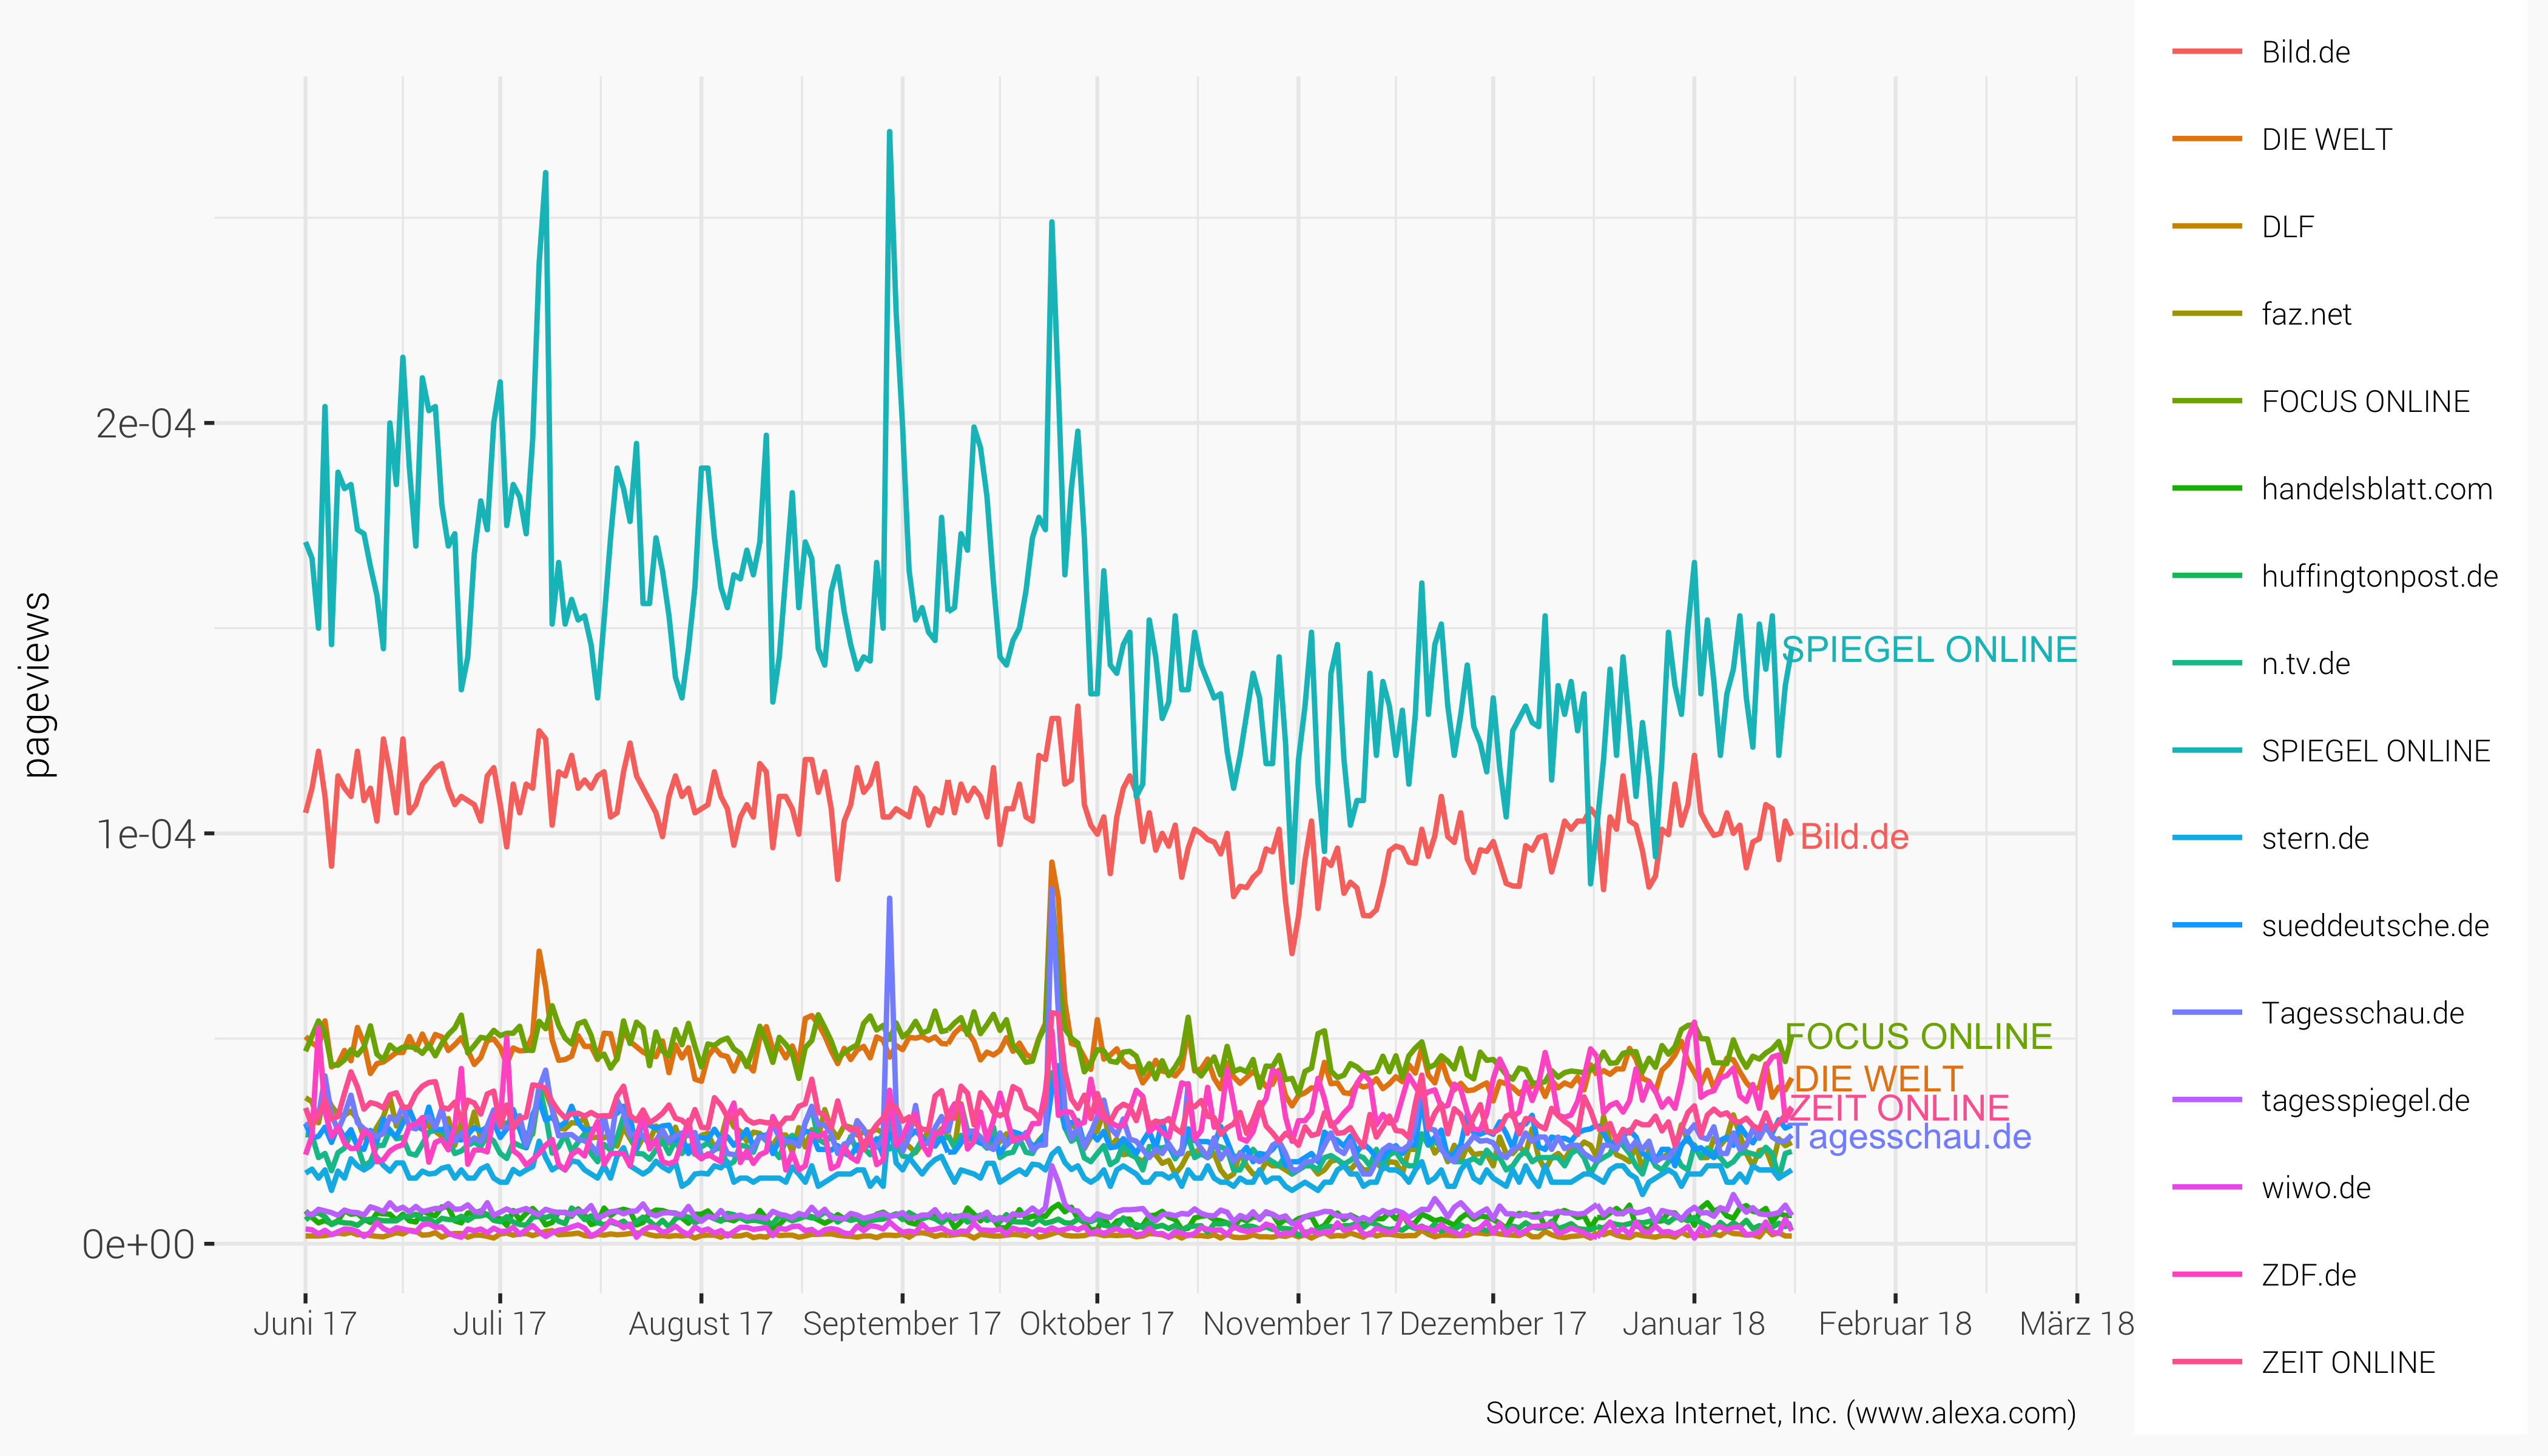
\includegraphics[width=\textwidth]{../figs/reach.png}
	\label{fig_reach}
\end{figure}

I conduct the estimation on a sample of 9,393 online news articles from six news provider about domestic politics\footnote{Bild.de, DIE WELT, FOCUS ONLINE, SPIEGEL ONLINE, ZEIT ONLINE, Tagesschau.de}, of which only Tagesschau.de belongs to the group of public provider. The reason for this is that the content structure of Tagesschau.de is most similar to that of the private providers. ZDF.de offers predominantly video content and DLF website mainly offers audio content in the form of interviews, which makes it hard to include it in the model. However, as only a part of the private suppliers are included to maintain the proportions between private and public market participants are maintained, thus minimizing possible bias. The articles are dated from 01.06.2017 to 31.12.2017.\footnote{German federal elections took place on 24th of September 2017.} I first extract all online articles using the the Webhose.io API.\footnote{For more information see https://docs.webhose.io/v1.0/docs/getting-started. The scraping code was written in Python and can be made available on request.} Then all articles from the section "domestic policy" are filtered by checking the URL structure.

Figure \ref{fig_distr1} shows the distribution of the number of articles from the respective news sources by date. There is a high peak around the federal elections on September, 24th.  

\begin{figure}[H]
	\caption{Article distribution...}
	\begin{center}
		\begin{subfigure}[normla]{0.49\textwidth}
			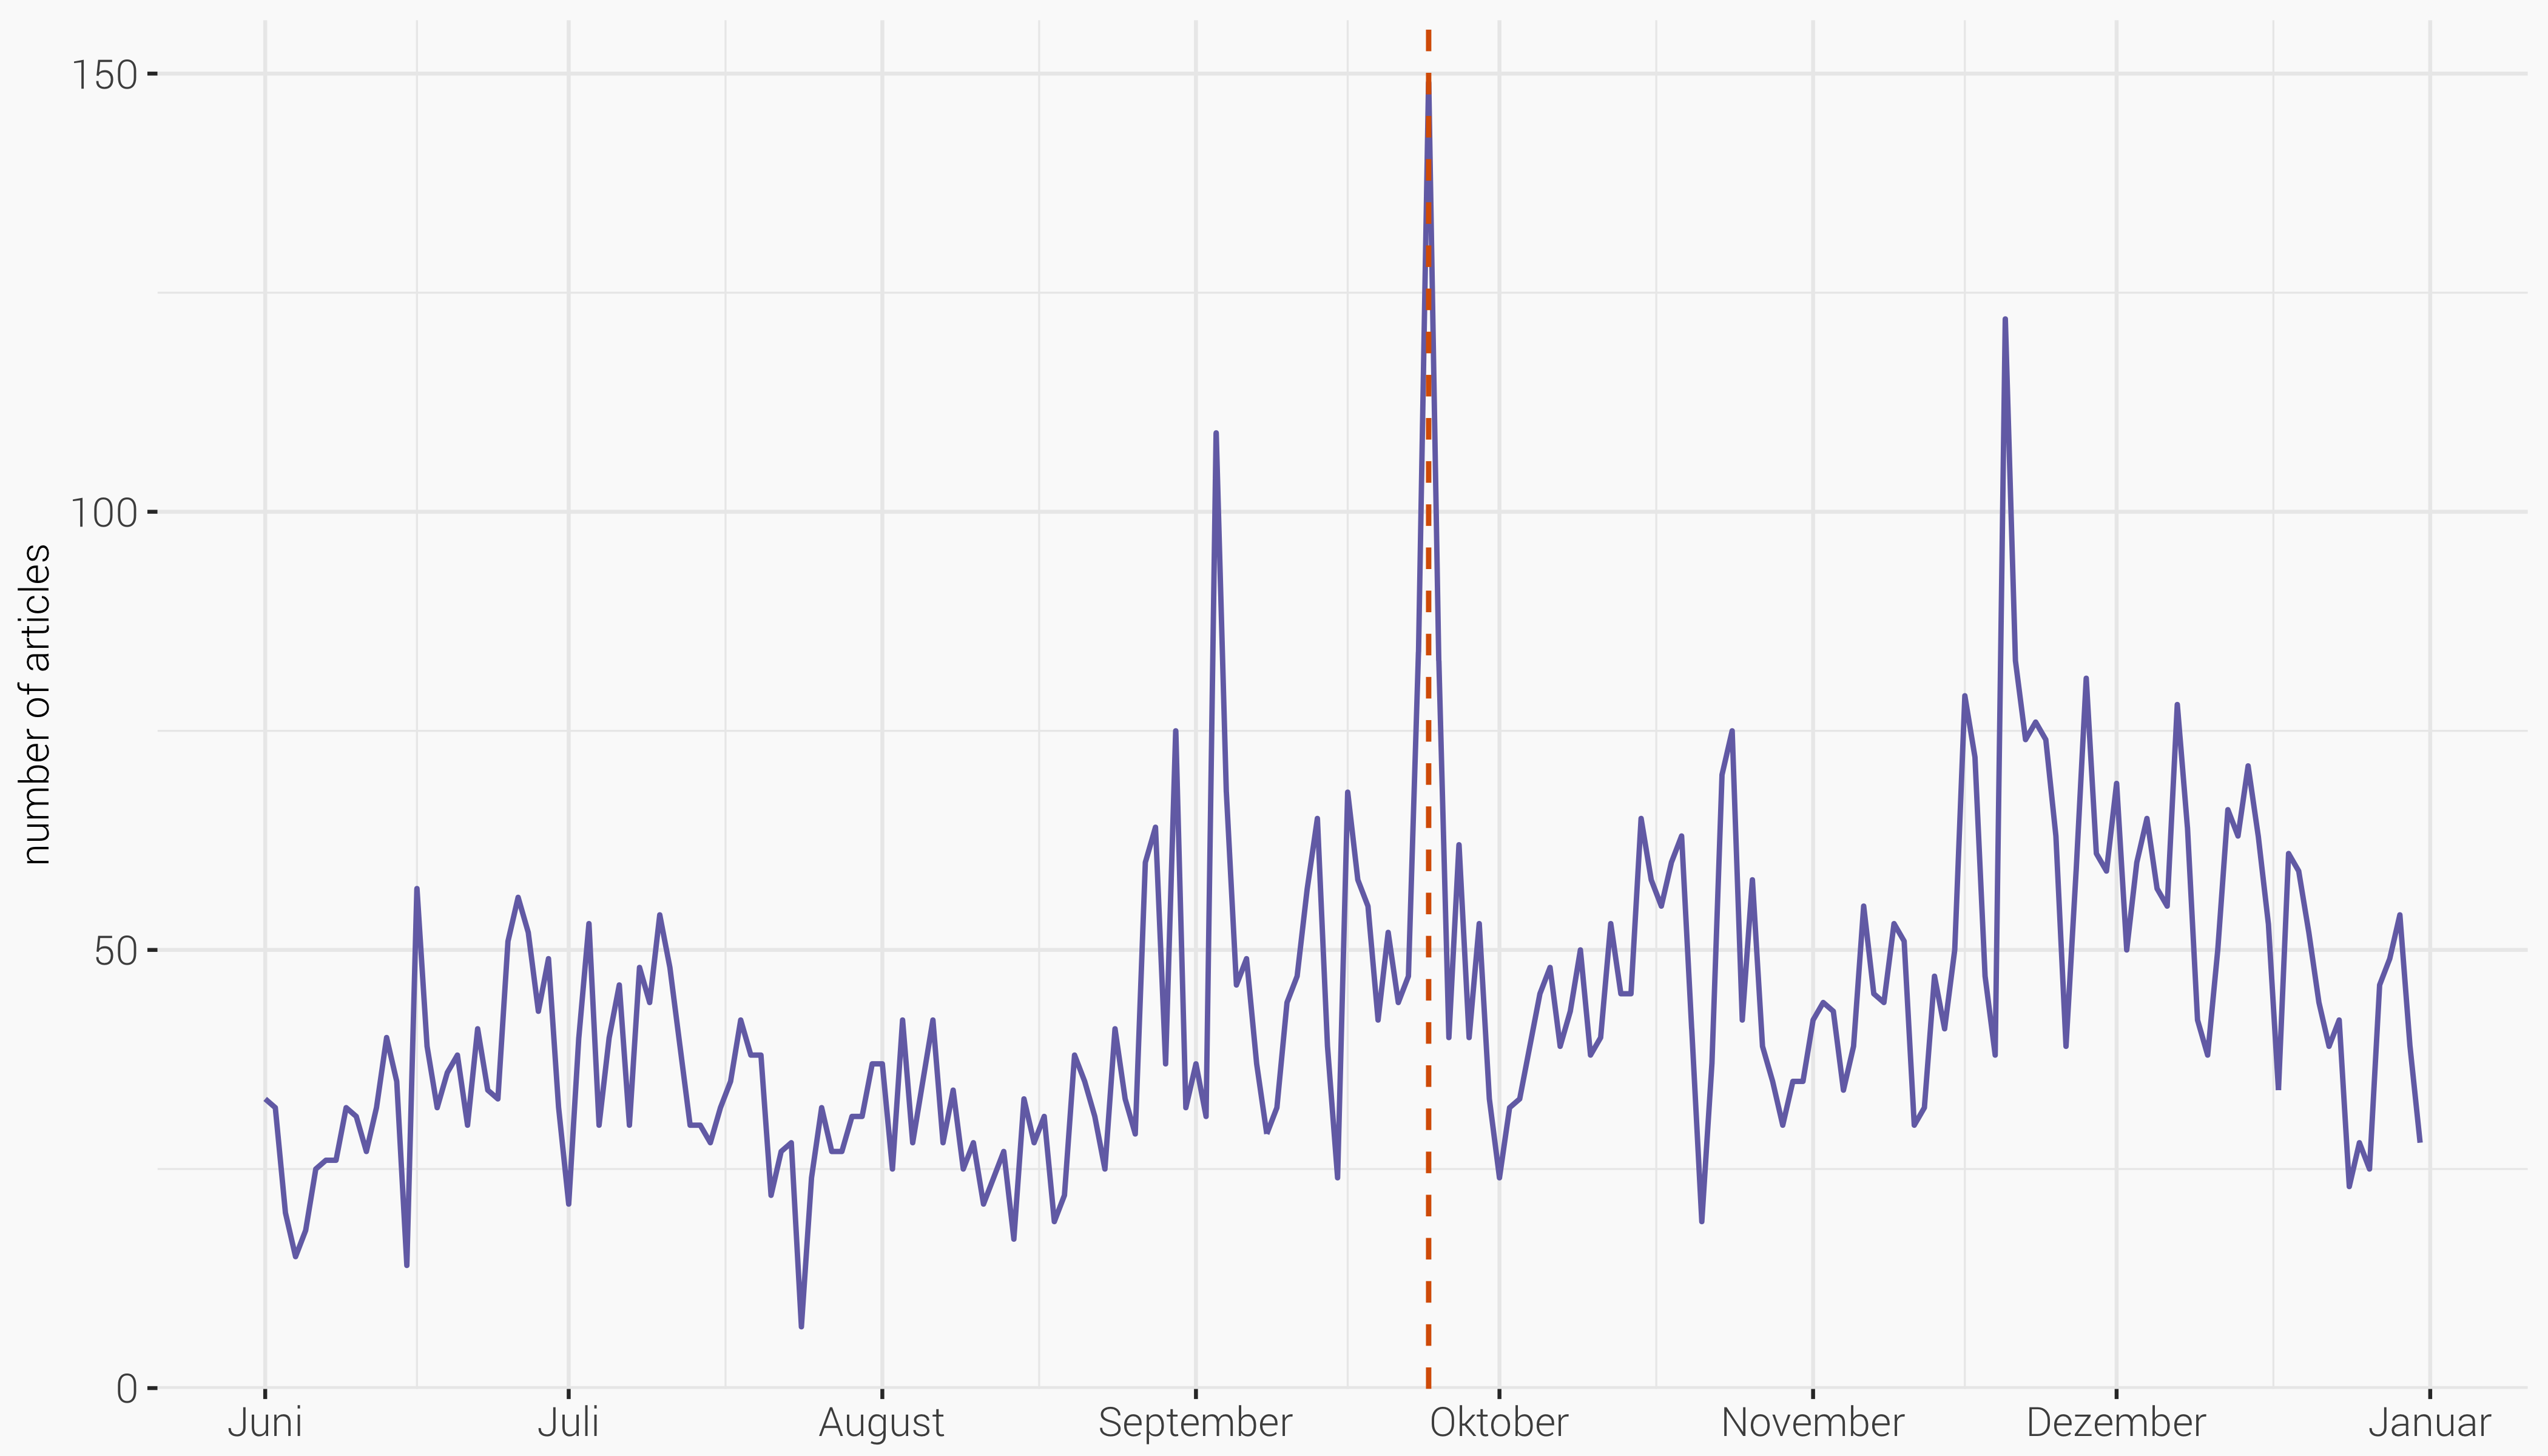
\includegraphics[width=\textwidth]{../figs/timeline.png}
			\caption{...by date}
			\label{fig_distr1}
		\end{subfigure}
		\begin{subfigure}[normla]{0.49\textwidth}
			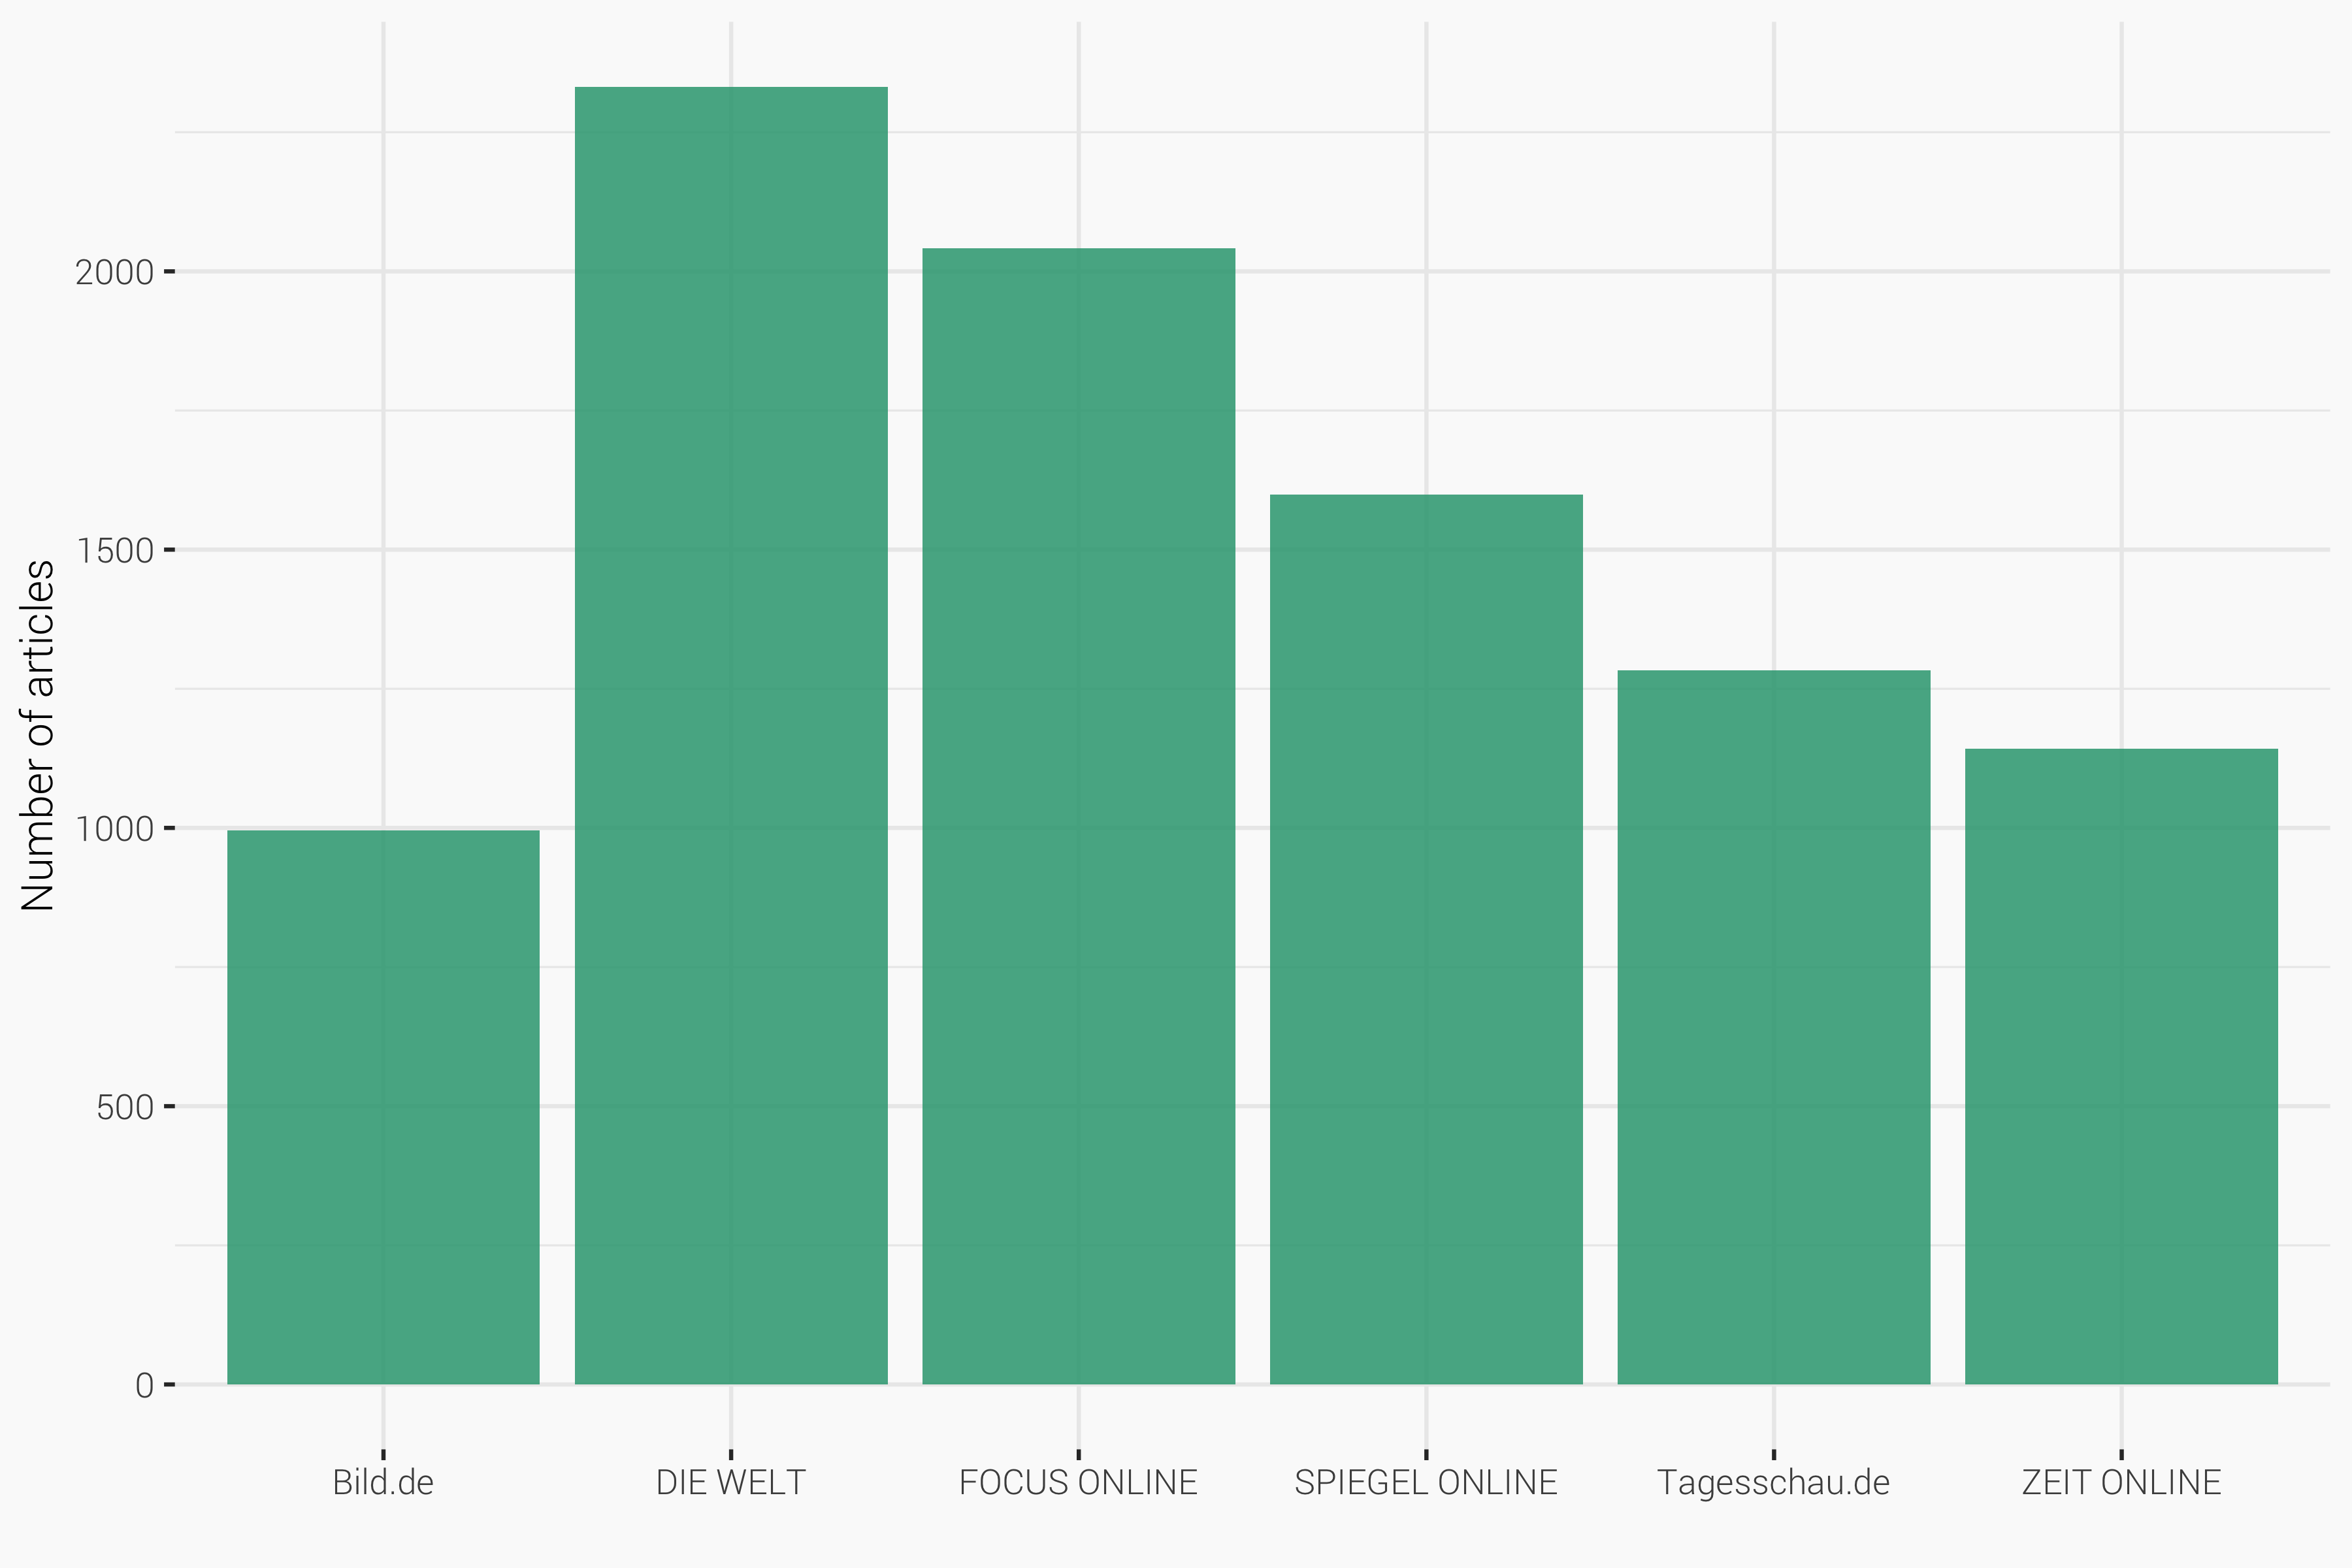
\includegraphics[width=\textwidth]{../figs/bar.png}
			\caption{... by news source}
			\label{fig_distr2}
		\end{subfigure}
	\end{center}
\end{figure}

% ------------------
% Text Pre-Procesing
% ------------------

A central task in text mining is to extract low-dimensional information from documents that are high-dimensional by nature \citep{bholat_text_2015}. This is related to the task of reducing the number of unique language elements in order to reduce the dimensionality of data (to avoid unnecessary computational complexity and overfitting) while at the same time keeping those words that reflect the content of a document. Any useful representation of text will throw away some information, the trick is to include the relevant information for our needs, and exclude the extraneous information. A common strategy to use text as data and reduce the dimensionality, is to pre-process the text by imposing some preliminary restrictions (stop-word removal, tokenization) based on the nature of the data (twitter text, newspaper articles, speeches, etc.) to reduce the number of language elements \citep{gentzkow_text_2017}. Intuitively the term frequency (tf) of a word is a measure of how important that word may be. There are words in a document, however, that occur many times but may not be important like articles, conjunctions, and so on. These terms, often called "stop words", are important to the grammatical structure of a text, but typically don't add any additional meaning and can therefore be neglected. We use a pre-defined stop word list from the Snowball stemmer project\footnote{http://svn.tartarus.org/snowball/trunk/website/algorithms/*/stop.txt} together with a customized list of stop-words that are redundant superfluous or distorting. We also remove punctuation character (e.g. ., ,, !, ?, etc.) and all numbers from our corpus. After completing this steps we were left with 55.235 unique terms in our vocabulary.

After pre-processing, each document $d$ is a finite list of terms. Each unique term in the corpus is indexed by some $v \in \lbrace 1,...,V \rbrace$ where $V$ is the number of unique terms. For each document $d \in \lbrace 1,...,D \rbrace$ we compute the number of occurrences of term $v$ in document $d$ to obtain the count $x_{d,v}$. The $D$ x $V$ matrix $\boldsymbol{X}$ of all such counts is called the document-term matrix. This representation is often referred to as the bag of words model, since the order in which words are used within a document is completely disregarded. 

% ----------------------
% Structural topic Model
% ----------------------
\section{The structural topic model}\label{ch_model}

The structural topic model (STM) developed by \citet{roberts_model_2016} allows to incorporate document specific covariates (e.g. the author or date of a document). STM is a recent extension of the standard topic modeling technique, labeled as "latent Dirichlet allocation" (LDA), which refers to the Bayesian model in \citet{blei_latent_2003} that treats each word in a topic and each topic in a document as generated from a Dirichlet - distributed prior.\footnote{See also \citet{griffiths_probabilistic_2002}, \citet{griffiths_finding_2004} and \citet{hofmann_probabilistic_1999}. \citet{pritchard_inference_2000} introduced the same model in genetics for factorizing gene expression as a function of latent populations.} Topic models formalize the idea that documents are formed by hidden variables (topics) that generate correlations among observed terms. Since its introduction into text analysis, LDA has become hugely popular and especially useful in political science.\footnote{see \citet{blei_probabilistic_2012}, \citet{grimmer_text_2013} and \citet{wiedmann_text_2016} for an overview in social science and \citet{gentzkow_text_2017} give an overview of text mining applications in economics.} \citet{wiedmann_text_2016} uses topic model methods on large amounts of news articles from two german newspapers published between 1959 and 2011, to reveal how democratic demarcation was performed in Germany over the past six decades. \citet{paul_cross-collection_2017} compares editorial differences between media sources, using cross-collection latent Dirichlet allocation (ccLDA), an LDA-based approach that incorporates differences in document metadata. They use a dataset of 623 news articles from August 2008 from two American media outlets - msnbc.com and foxnews.com - to compare how they discuss topics. Reviewing the top words of the word-topic distribution, they find some content differences between the two. 

STM has been applied to multiple academic fields: \citet{roberts_structural_2014} uses STM to analyse open-ended responses from surveys and experiments, \citet{farrell_corporate_2016} applies the model to scientific texts on climate change, revealing links between corporate funding and the framing of scientific studies. \citet{mishler_using_2015} show that "STM can be used to detect significant events such as the downing of Malaysia Air Flight 17" when applied to twitter data. Another study shows how STM can be used to explore the main international development topics of countries’ annual statements in the UN General Debate and examine the country-specific drivers of international development rhetoric \citep{baturo_what_2017}. \citet{mueller_reading_2016} use newspaper text to predict armed conflicts in different regions. They use the estimated topic shares in linear fixed effects regression to forecast conflict out-of-sample. \citet{roberts_navigating_2016} use STM to examine the role of partisanship in topical coverage using a corpus of 13,246 posts that were written for 6 political blogs during the course of the 2008 U.S. presidential election. With the aim of revealing the effect of partisan membership on topic prevalence, each blog is assigned to be either liberal or conservative. To explore the differences between the two, they look at the expected proportion of topic and examine the posts most associated with a respective topic. This approach is similar to \citet{roberts_model_2016}. They also use different measures of distance between the topic-word distributions of the same topic within different models. In section \ref{ch_similarity} a similar approach is applied to measure similarity between the same topic for different covariate levels.

% Topic Modeling
% --------------
\subsection{Generative Process of STM}\label{ch_generativeProcess}

As mentioned above, the STM allows to incorporate observed document metadata which is able to affect both topical prevalence and topical content. The following description of the generative model - the process of filling a word-position in a document - of the STM is based on \citet{roberts_structural_2013} and \citet{roberts_stm:_2016}. For each document $d$ and a given number of topics $K$, a document-specific topic-prevalence vector $d(\boldsymbol{\theta}_d)$ is drawn from a logistic-normal distribution, where the parameters are a function of the covariate values:

\begin{equation}
	\boldsymbol{\theta}_d|\boldsymbol{x}_{d\gamma},\boldsymbol{\Sigma} \sim \textrm{LogisticNormal}(\mu = \boldsymbol{x}_{d\gamma}\boldsymbol{\Sigma}).
\end{equation}

$\boldsymbol{x}_d\gamma$ lists the values of all metadata covariates for document $d$, where $\gamma$ relates these covariate values to the topic-prevalence. The structure of $\boldsymbol{\Sigma}$ implies the possibility of correlations across documents in the topic-prevalence vector. 

According to $\theta$, a specific topic $z_{dn}$ is assigned for the $n^{th}$ word-position in the document through the process:

\begin{equation}
	z_{dn}|\boldsymbol{\theta}_d \sim \textrm{Multinomial}(\boldsymbol{\theta}_d).
\end{equation}

Conditional in the topic chosen, a specific word, $w_{dn}$, is chosen from the overall corpus vocabulary $V$, using the following process:

\begin{equation}
	w_{dn}|z_{dn},\beta_{dkv} \sim \textrm{Multinomial}(\beta_{dk1},...,\beta_{dkV}),
\end{equation}

where the word probability $\beta_{dkv}$ is parameterized in terms of log-transformed rate deviations from the rates of a corpus-wide background distribution $m_v$. The log-transformed rate deviations can then be specified by a collection of parameters $\lbrace \boldsymbol{\kappa} \rbrace$, where $\kappa^{(t)}$ is a $K$-by-$V$ matrix containing the log-transformed rate deviations for each topic $k$ and term $v$, over the baseline log-transformed rate for term $v$. This matrix is the same for all $A$ levels of covariates. To put it differently, $\kappa^{(t)}$ indicates the importance of the term $v$ given topic $k$ regardless of the covariates. Similarly, $\kappa^{(c)}$ is a $A$-by-$V$ matrix, indicating the importance of the term $v$ given the covariate level $c$ regardless of the topic. Finally, $\kappa^{(i)}$ is a $A$-by-$K$-by-$V$ matrix, collecting the covariate-topic effects:

\begin{equation}
	\beta_{dkv}|z_{dn}=\frac{\textrm{exp}(m_v+\kappa^{(t)}_{kv},\kappa^{(c)}_{y_dv}+\kappa^{(i)}_{y_dkv})}{\sum_v \textrm{exp}(m_v+\kappa^{(t)}_{kv},\kappa^{(c)}_{y_dv}+\kappa^{(i)}_{y_dkv})}.
\end{equation}

The STM maximizes the posterior likelihood that the observed data were generated by the above data-generating process using an iterative approximation-based variational expectation-maximization algorithm\footnote{A technical description of this maximization process can be found in \citet{roberts_model_2016}} available in R's stm package \citep{roberts_stm:_2016}. The process gives us two posterior distribution parameter: (1) $\beta$ is a $K$-by-$V$ matrix (where $K=$ number of topics and $V=$ vocabulary), where the entry $\beta_{kvc}$ can be interpreted as the probability of observing the $v$-th word in topic $k$ for the covariate level $c$. (2) $\theta$ is a $D$-by-$V$ matrix of the document-topic distributions, where the entry $\theta_{dk}$ can be interpreted as the proportion of words in document $d$ which arise from topic $k$, or rather as the probability that document $d$ deals about topic $k$. These probability distributions are used to compare the content of public and private news providers in section \ref{ch_empirical}.


% ----------------------
% Model Selection
% ----------------------
\subsection{Model and parameter selection}

Inference of mixed-membership models, such as the one applied in this paper, has been a thread of research in applied statistics in the past few years \citep{blei_latent_2003} \citep{erosheva_mixed-membership_2004} \citep{braun_variational_2010}. Topic models are usually imprecise as the function to be optimized has multiple modes, such that the model results can be sensitive to the starting values. Since an ex ante valuation of a model is hardly possible, I compute a variety of different models and compare their posterior probability. This enables me to check how results vary for different model solution \citep{roberts_navigating_2016}. I then cross-checked some subset of assigned topic distributions to evaluate whether the estimates align with the concept of interest \citep{gentzkow_text_2017}. These manual audits are applied together with numeric optimization based on the topic coherence measure suggested by \citet{mimno_optimizing_2011}. 

This process revealed that a model with 40 topics best reflects the structure in the corpus. Furthermore, the ownership of the news provider of each article (public or private) and the month it was published are used as covariates in the topic prevalence. In other words, the probability distribution of topics depends on the business-model as well as on the month the article was published. The ownership is also included as a covariate affecting topical content, following the assumption that the same topic is discussed in different ways in private and public media respectively. To address problems due to non-convexity, we rely on the spectral initialization approach advocated by \citet{roberts_navigating_2016}. 

% ----------------------
% Model Results
% ----------------------
\section{Empirical Evaluation}\label{ch_empirical}

This section summarizes the results of the STM. Subsequently different measures to analyze the content differences between public and private ownership are applied according to the following approaches: (1) To address the question whether market imperfections exist in that sense, that some topics are not covered by private but by public news provider, I use the document-topic probability $\theta$, to estimate the conditional expectation of topic prevalence for given document characteristics (See section \ref{subsectiona_topicprevalence}). (2) Next, I find all edges between topics where they exhibit a positive correlation of $\theta$ above 0.1 to examine how topics are correlated differently for different covariate levels, indicating how topics are connected and framed differently between private and public media (see section \ref{subsection_topiccorrelation}). Approaches (1) and (2) have been used in \citep{roberts_model_2016}. However, we extend the analysis by (3) calculating the similarity of the word-topic distribution $\beta$ between the news provider using various distance measures, to identify which topics are discussed similar or differently (see section \ref{subsection_similarity}). 

In order to get an initial overview of the results, Figure \ref{fig_topic_proportion} displays the topics ordered by their expected frequency across the corpus (left side of the Figure) and the expected proportion of a topic in public media minus the expected proportion of topic use in private media (right side of the Figure). Thus topics more associated with public media appear to the right of zero. To assign a label to each topic, I looked at the most frequent words in that topic and the most representative articles \citep{roberts_model_2016}. 

It becomes apparent that the topic (topic 3) about the coalition talks between the so-called Jamaica parties (CDU/CSU, FDP and Bündnis 90/Die Grünen) is the topic with the highest expected frequency in the whole corpus, followed by the topics about refugees in Germany (topic 32) and the coalition talks between CDU/CSU and SPD (topic 1), that began shortly after the failure of the Jamaican coalition. Particularly in the latter case, there is no discernible difference between private and public providers, while topic 3 and 32 are more likely to be seen in public news. The biggest difference can be seen in Topic 23, which covers court proceedings, especially in relation to the NSU case. Private providers seem to be less likely to report on this topic, as it is of less likelihood of observing this topic in the corpus of private news. Topic 7, which deals with political trends in Germany, seems to be discussed more often in private than in public news.    

\begin{figure}[H]
	\begin{center}
	\caption{Expected topic proportion}
		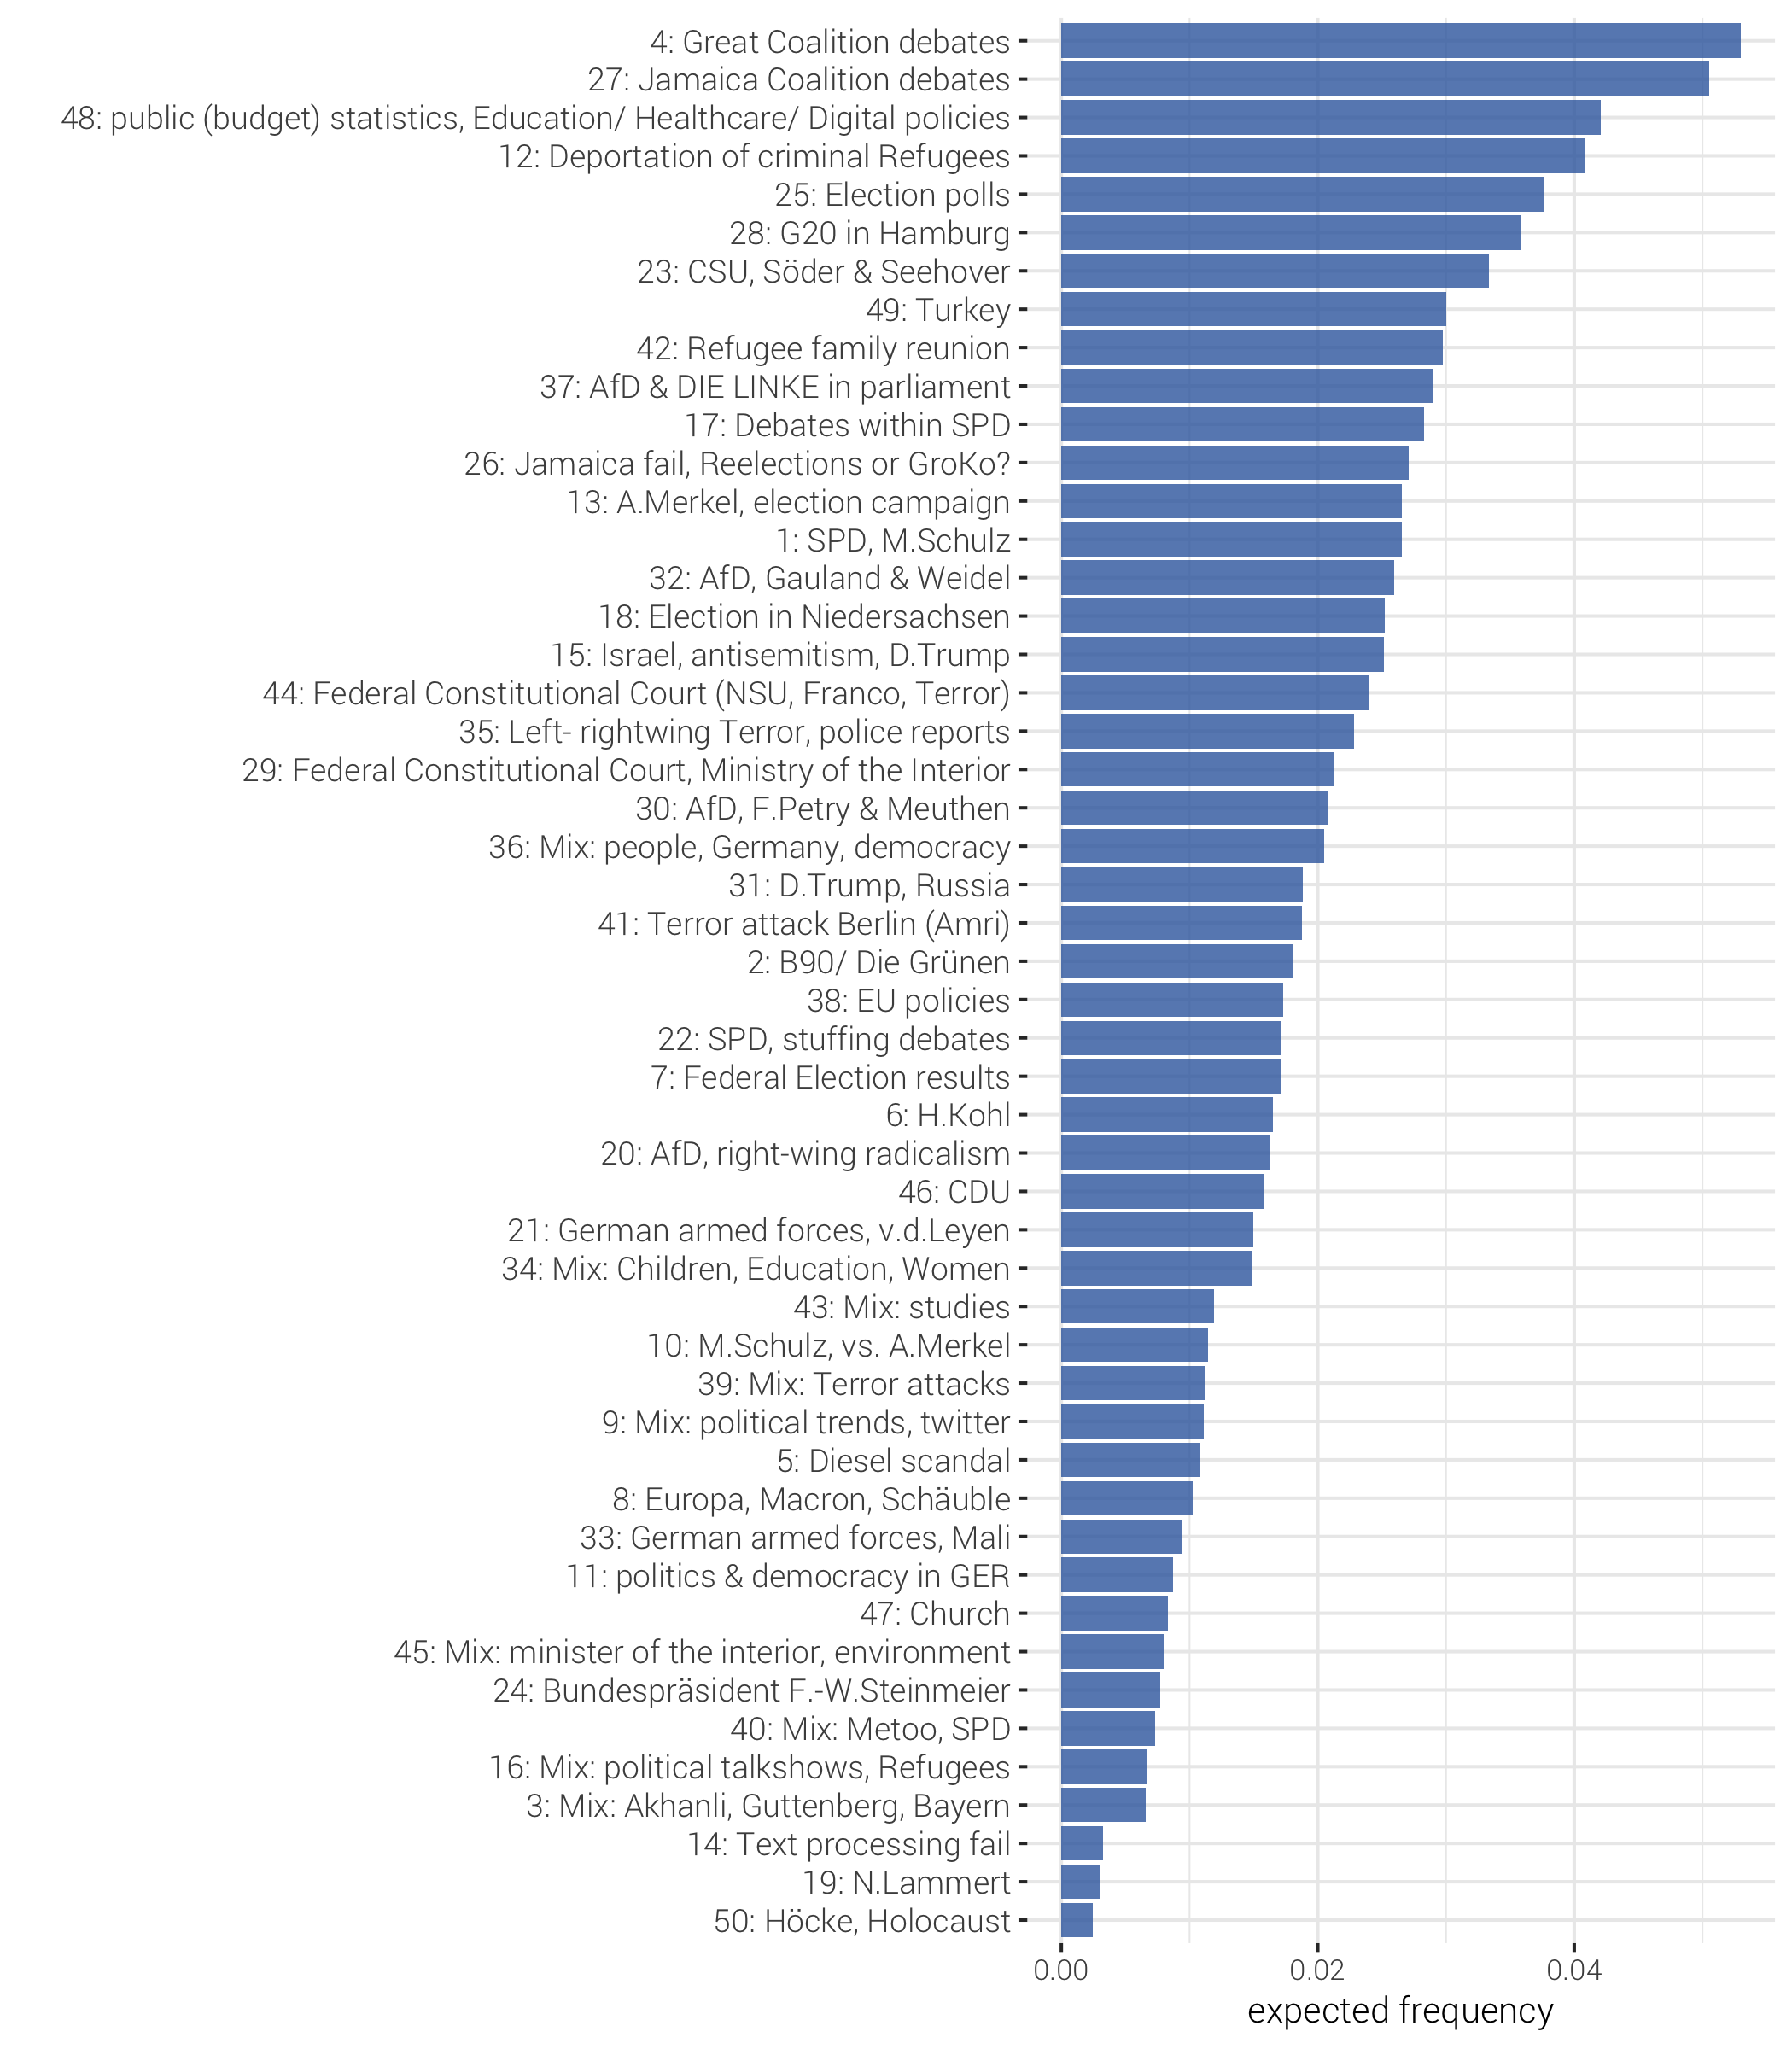
\includegraphics[width=\textwidth,keepaspectratio]{../figs/topic_proportion.png}
		\label{fig_topic_proportion}
\end{center}
\end{figure}

\subsection{Differences in topic prevalence}\label{subsectiona_topicprevalence}

To identify which of these differences is significant, the conditional expectation of topic prevalence for given document characteristics can be estimated \citep{roberts_model_2016}. More specifically, I estimate a linear model, where the documents are observations, the dependent variable is the posterior probability of a topic and the covariates are the metadata of documents (see equation \ref{eq_1}). The stm-package provides a function that uses the method of composition to incorporate uncertainty in the dependent variable, drawing a set of topic proportions from the variational posterior repeated times and compute the coefficients as the average over all results \citep{roberts_stm:_2016}.

\begin{equation}\label{eq_1}
	\theta_d=\alpha+\beta_1x_{ownership}+\beta_2x_{month}+\epsilon
\end{equation}

Figure \ref{fig_estimateEffects} displays the regression results for private vs. public. 

\begin{figure}[H]
	\caption{Regression results}
		\begin{center}
			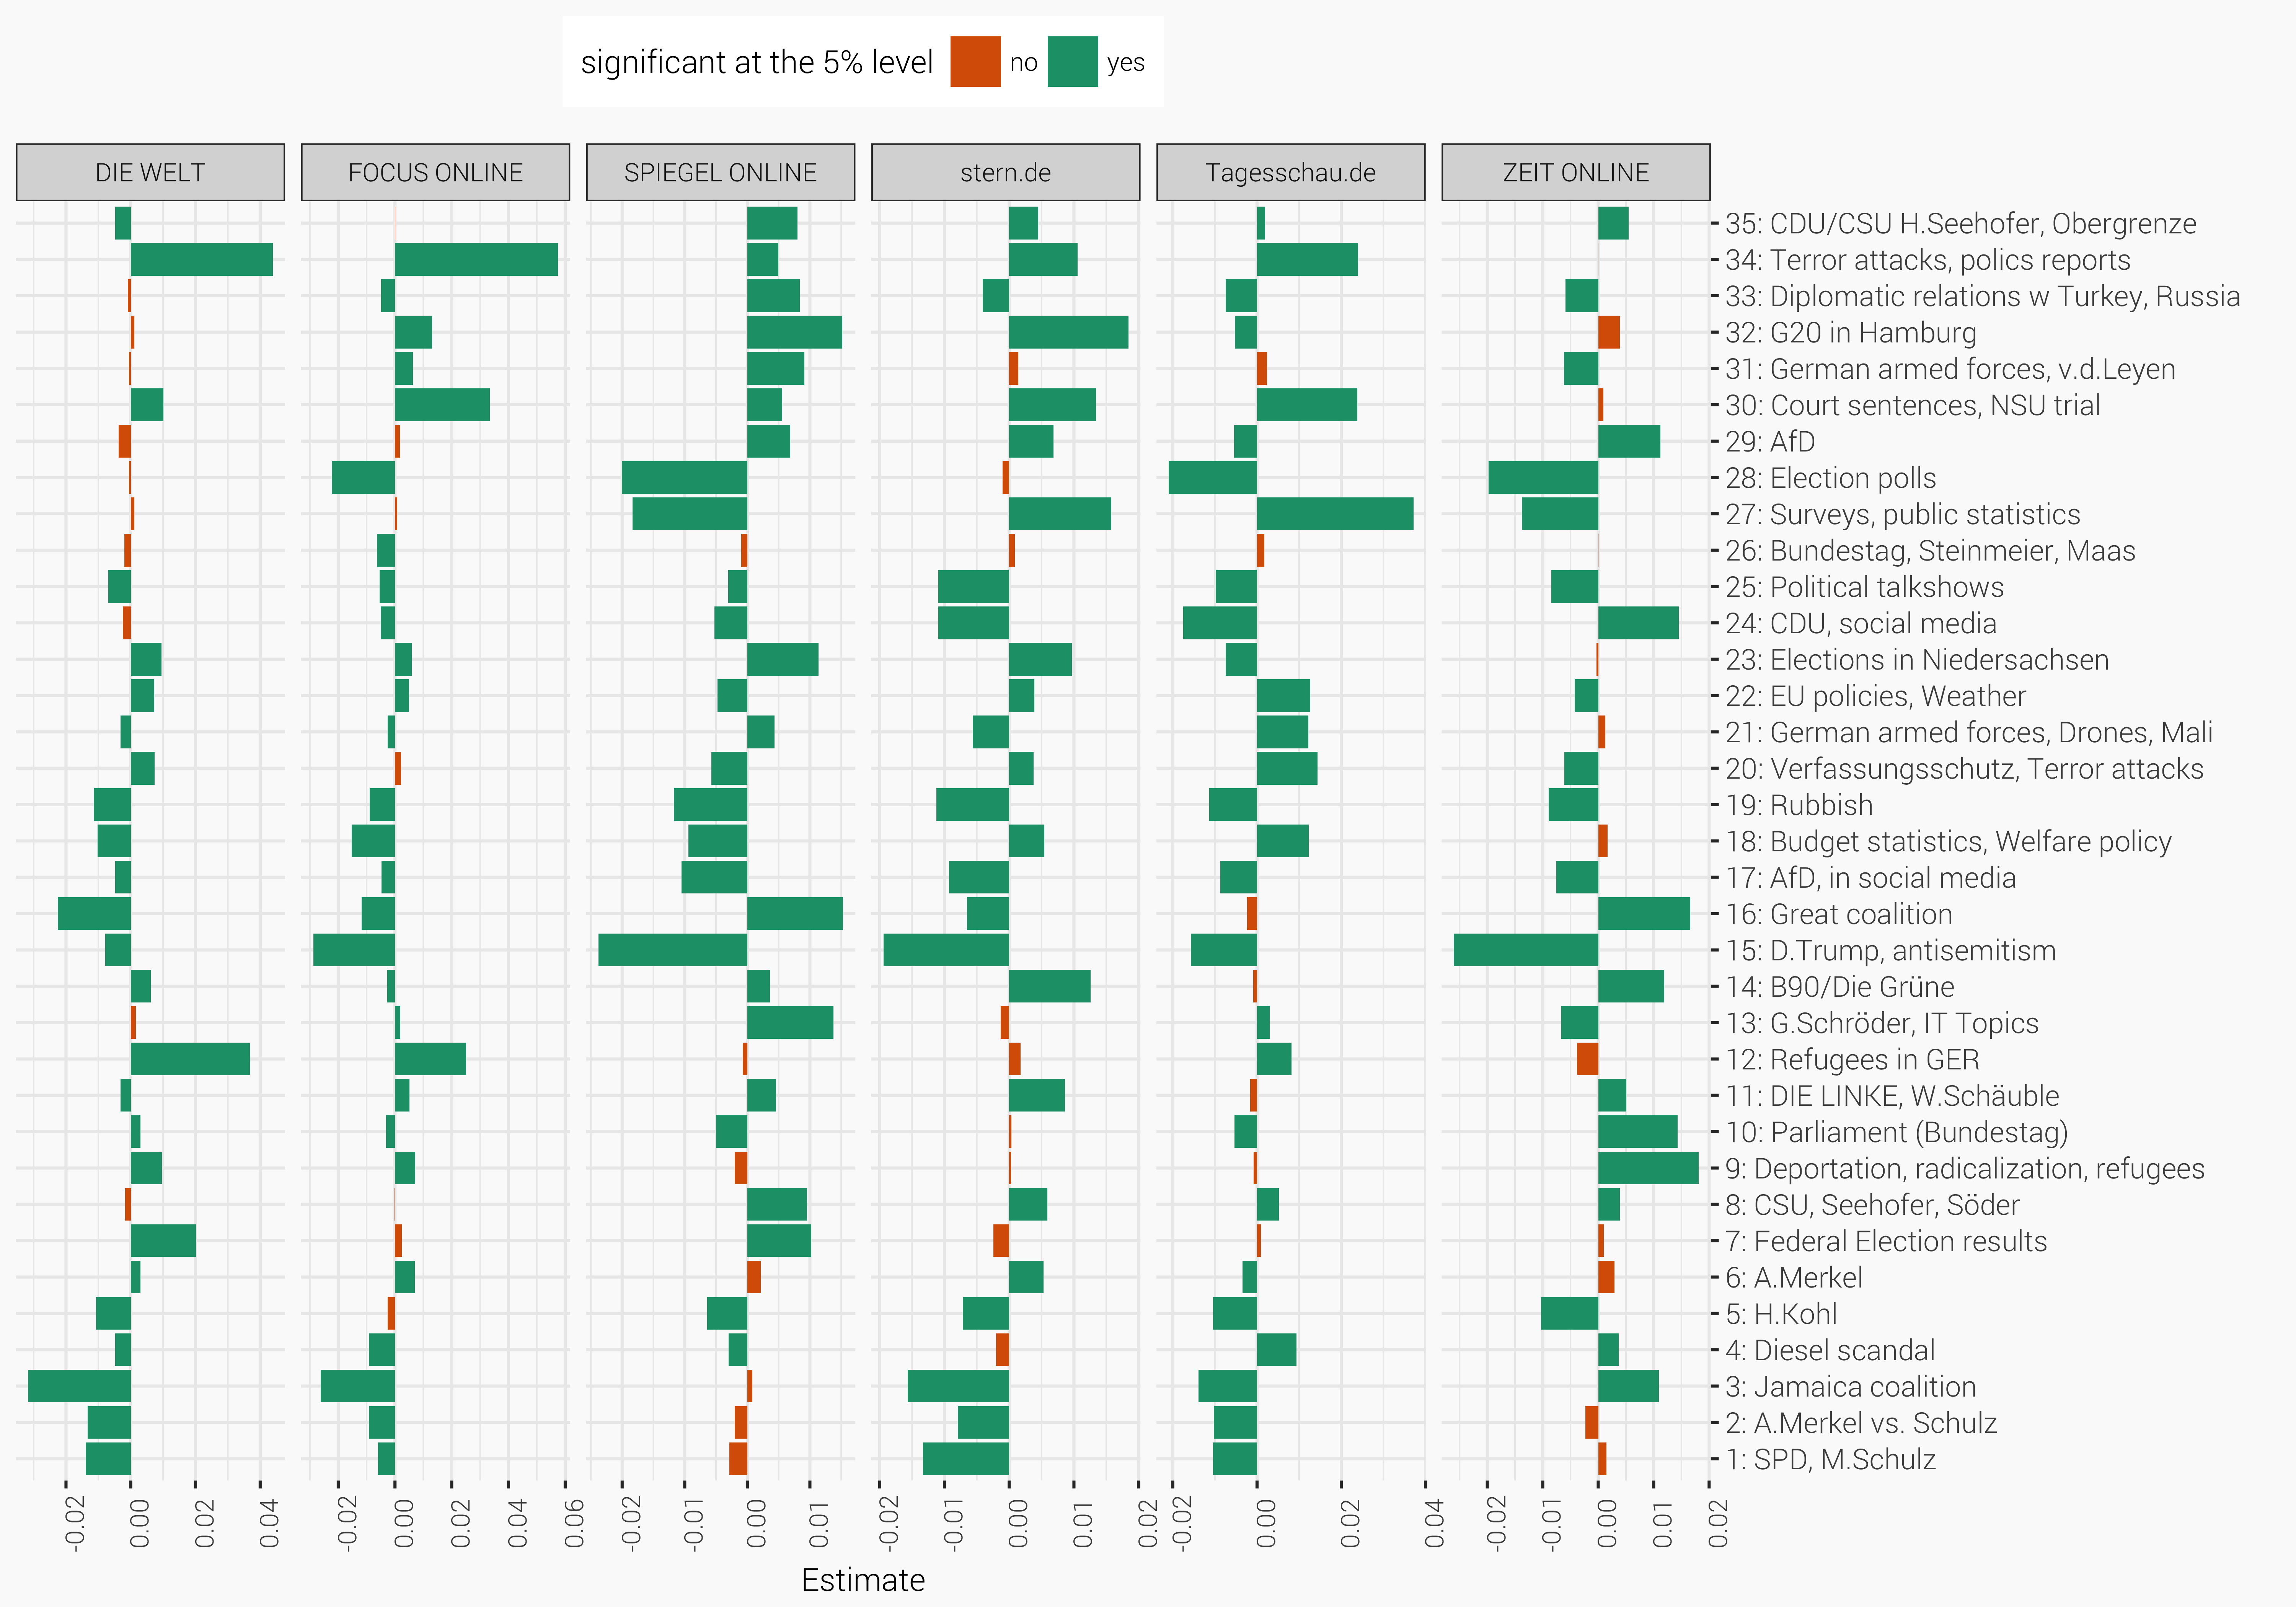
\includegraphics[width=0.9\textwidth,keepaspectratio]{../figs/estimates.png}
		\end{center}
	\label{fig_estimateEffects}
\end{figure}

\textcolor{red}{AUSWERTUNG}

\subsection{Topic correlations}\label{subsection_topiccorrelation}

Next, the topic correlation is calculated, indicating how topics are connected and framed in public and private media. In Figure \ref{fig_topic_correlations}, indicates all edges between topics where they exhibit a positive correlation above 0.1 \citep{roberts_model_2016}.


\begin{figure}[H]
	\caption{Topic Correlation}
		\begin{center}
		\begin{subfigure}{.7\textwidth}
			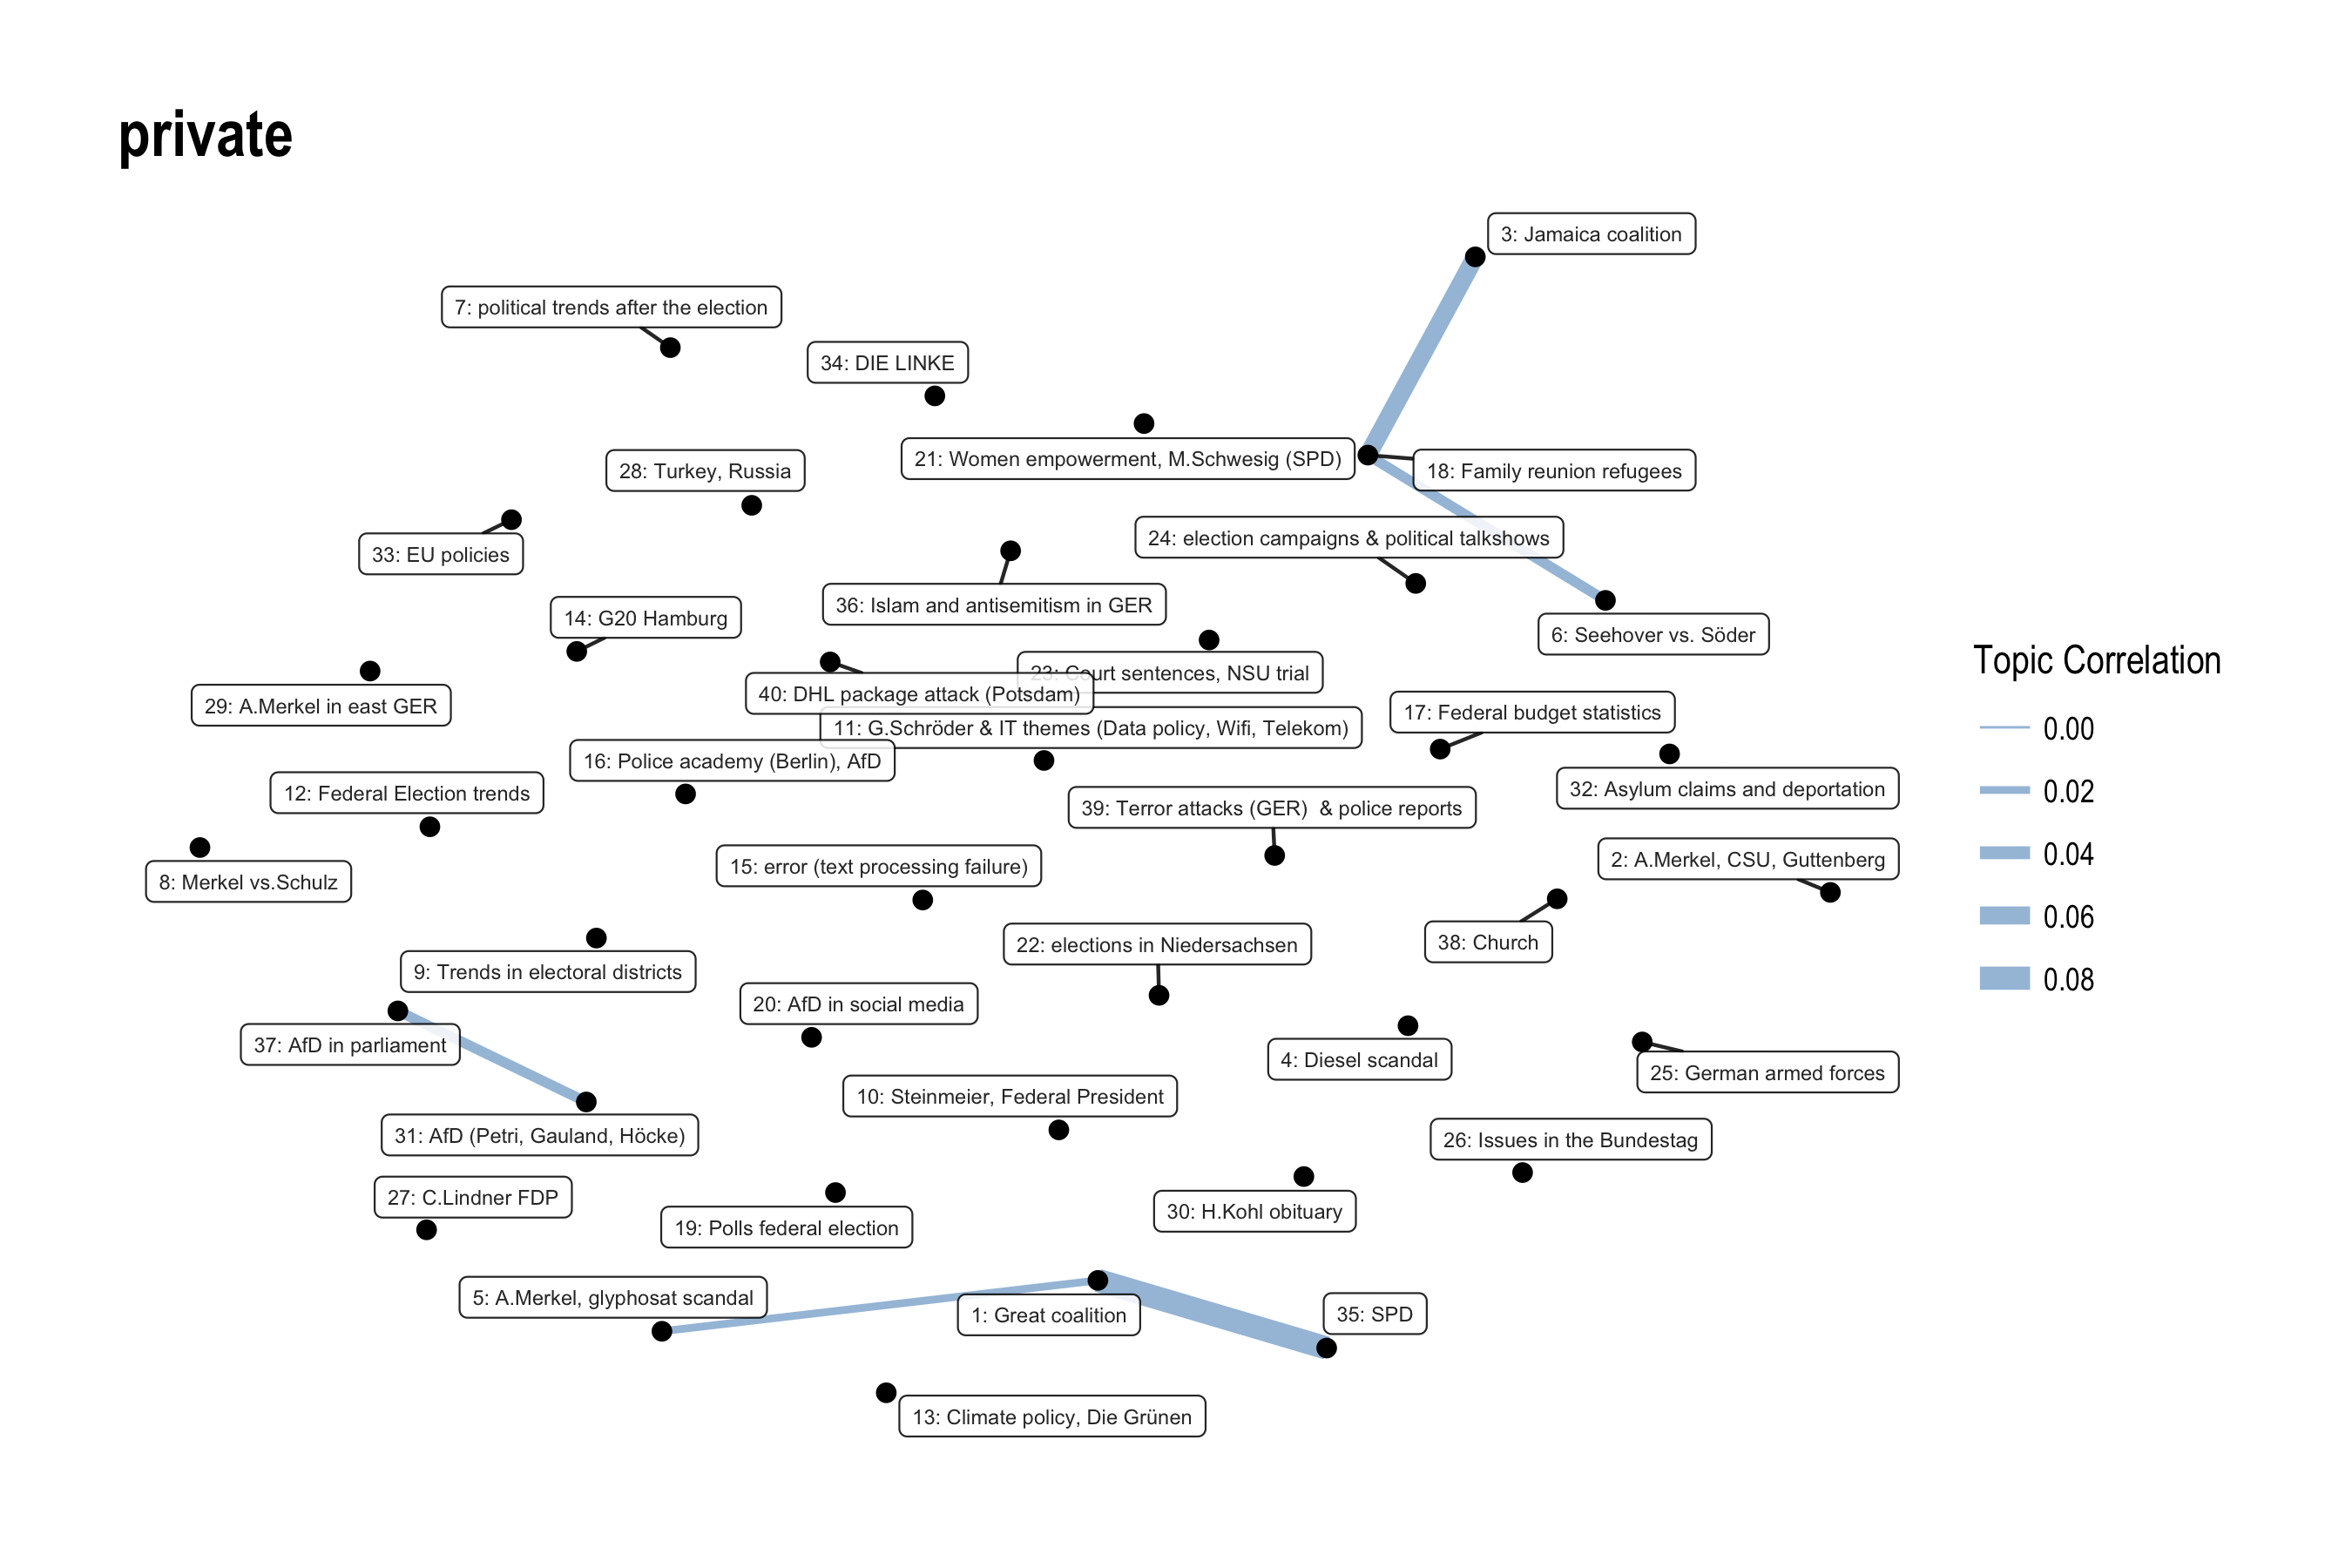
\includegraphics[width=\textwidth]{../figs/corrplot1.png}	
			\subcaption{Private news provider}
		\end{subfigure}
		\begin{subfigure}{.7\textwidth}
			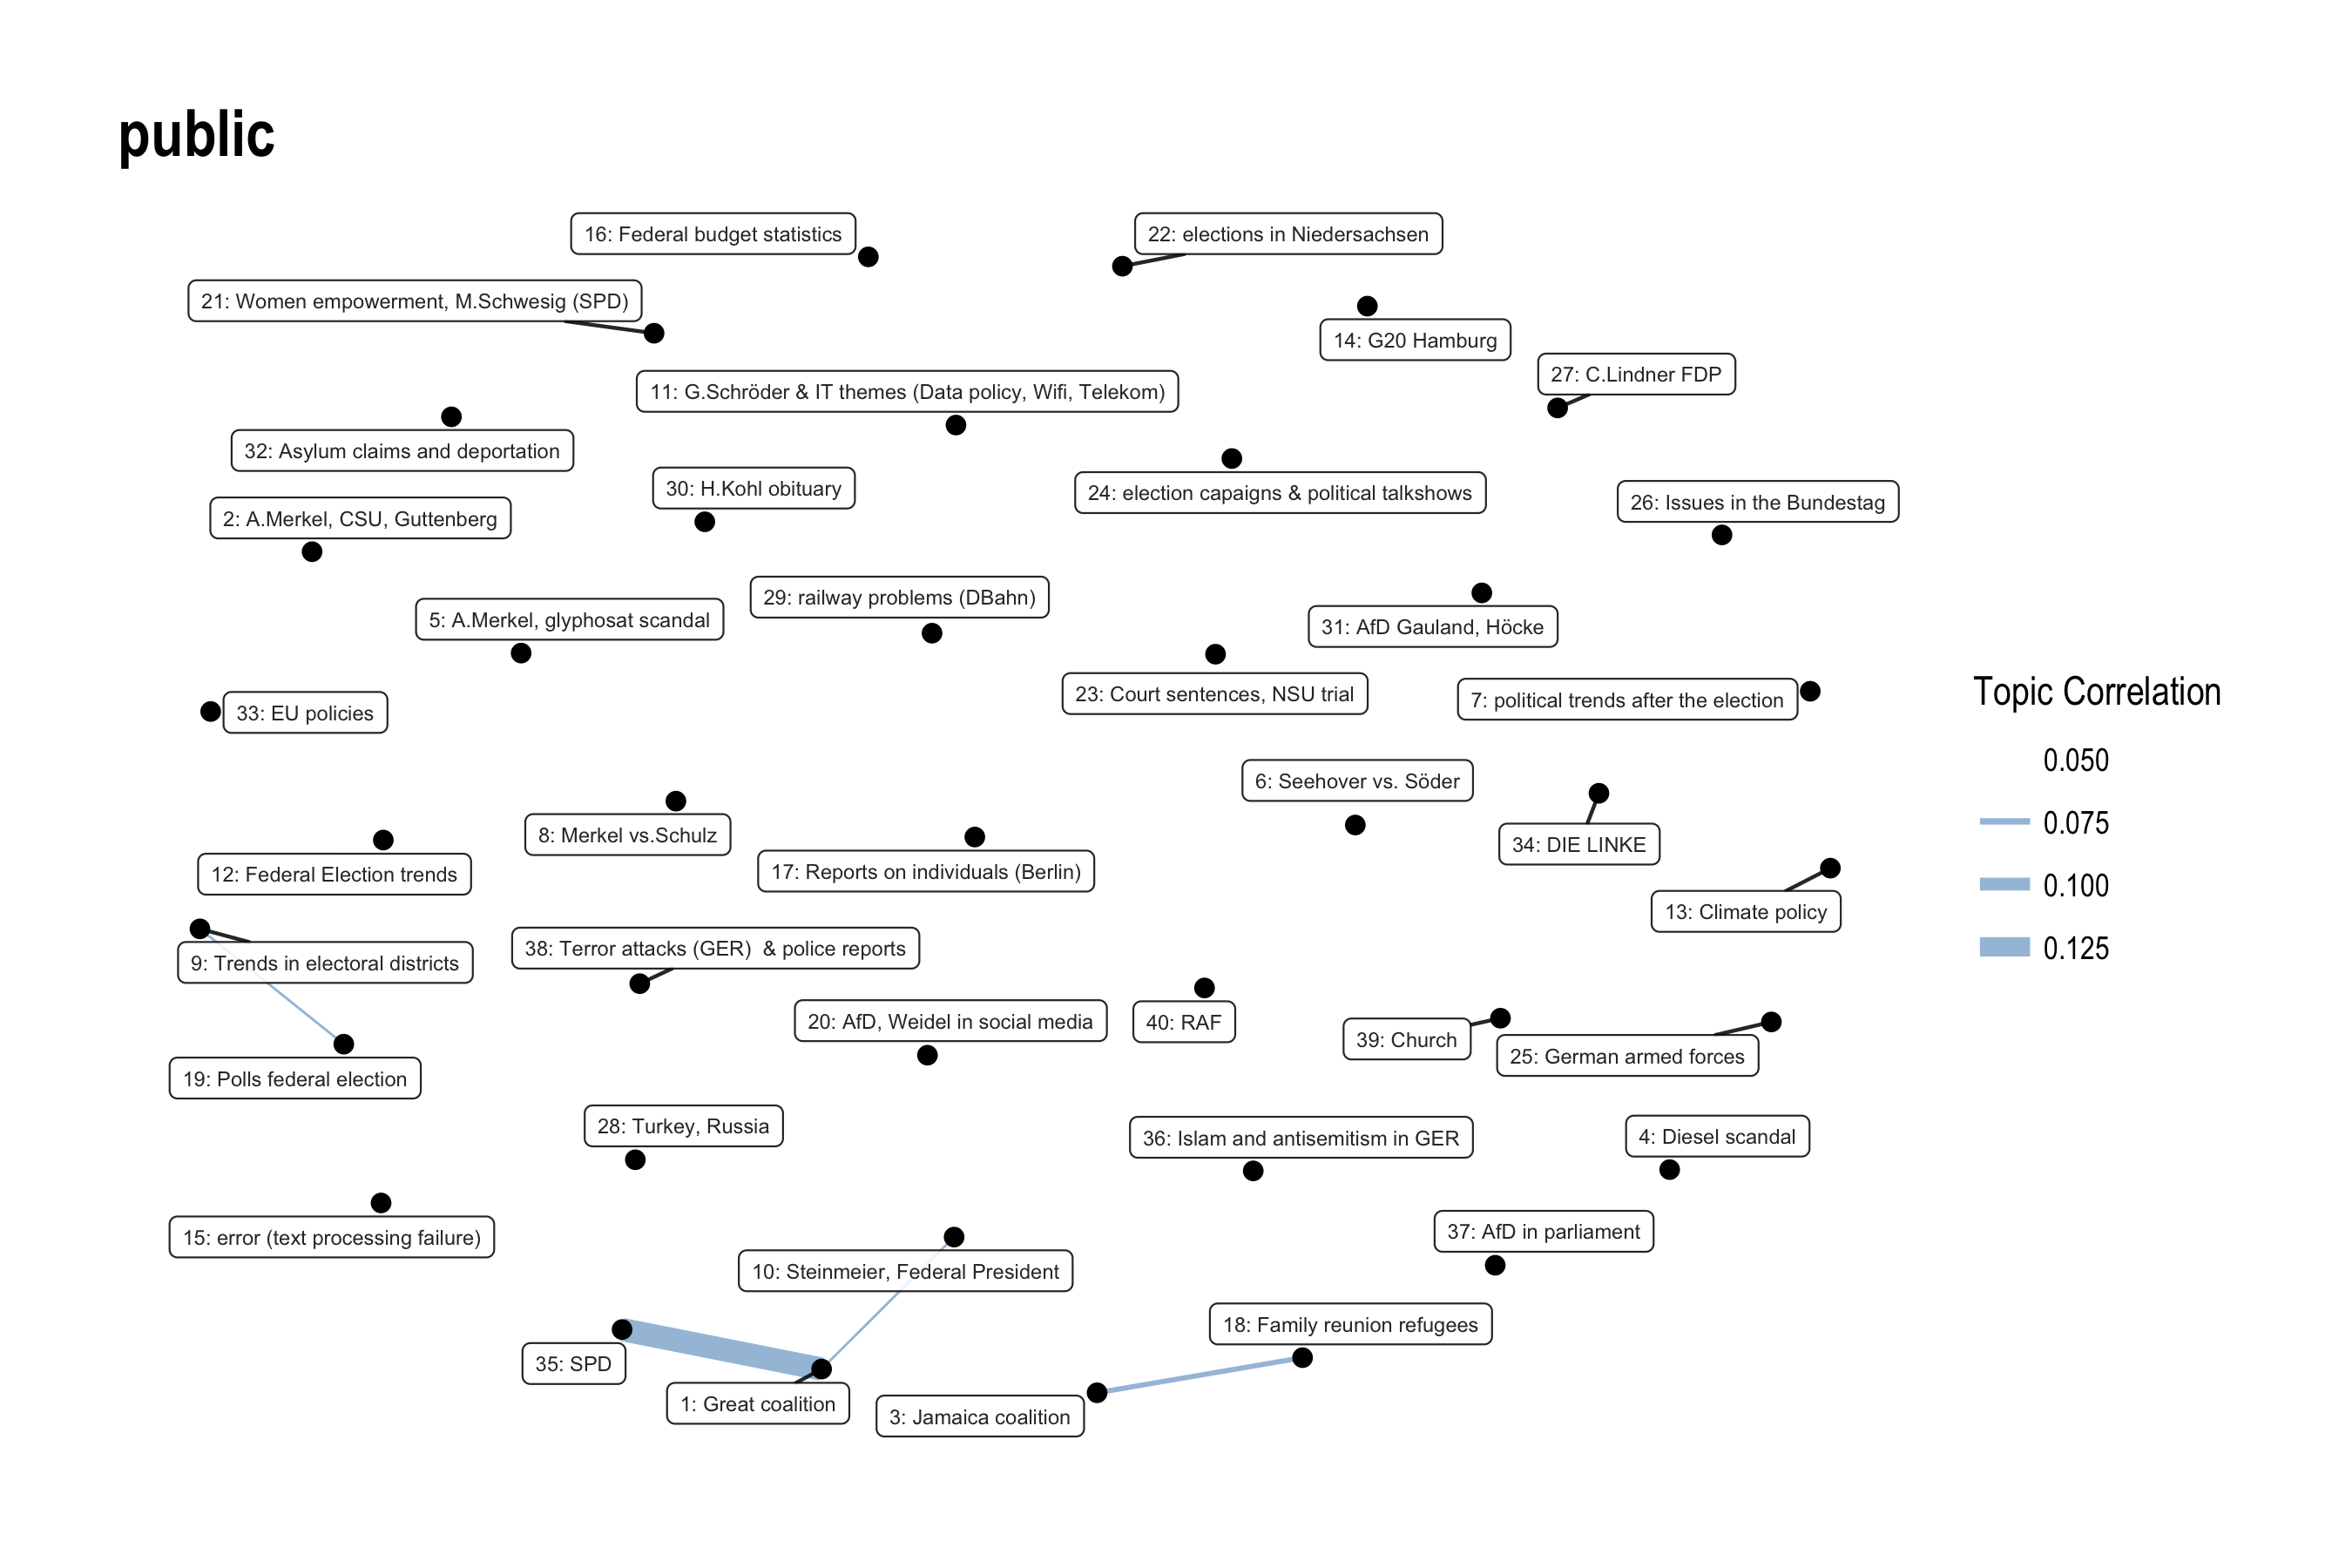
\includegraphics[width=\textwidth]{../figs/corrplot2}
			\caption{Public news provider}	
		\end{subfigure}
		\end{center}
	\label{fig_topic_correlations}
\end{figure}

\textcolor{red}{AUSWERTUNG}

\subsection{Differences in word-topic distributions}\label{subsection_similarity}

Previous topic modeling research try to measure the similarity between topics, comparing the word-topic-distribution between the topics (most of the research uses LDA without metadata, so the word-topic-distribution is the same within the whole corpus). cosine similarity \citep{he_detecting_2009}, \citep{ramage_labeled_2009}, Kullback-Leibler (KL) \citep{newman_distributed_2009}, \citep{wang_mining_2009} and the average Log Odds Ratio \citep{chaney_visualizing_2012} are frequently used metrics to compare word probability distributions. \citet{kim_topic_2011} compare six popular similarity metrics in terms of log likelihood of data, concluding that Jensen-Shannon Divergence (the symmetric variation of KL divergence) is best in terms of performance and generality. 

Since a topic is a multinomial distribution over the vocabulary, where $\beta_{kvi}$ indicates the probability of observing word $v$ in topic $k$ for covariate level $i$, we can analyze how similar a topic $k$ is for different levels of covariates. More precisely, we can calculate the similarity between $\beta_{kvi}$ and $\beta_{kvj}$. I use each row of that matrix (corresponding to each topic) to calculate the similarity of the word-topic distribution between the public and private media using the square root of the Jensen-Shannon (JS) Divergence. I will compare this metric with a set of other similarity measures recently used in the literature to measure the difference between word-topic distributions: The Kullback-Leibler (KL) divergence (\citet{newman_distributed_2009}, \citet{wang_mining_2009}), the cosine similarity (\citet{he_detecting_2009}, \citet{ramage_labeled_2009}) and the difference of the $L1$ norm of the vectors \citep{roberts_navigating_2016}. Before the results are presented, I will briefly explain these measures before I proceed to the results.

Essentially, the KL divergence is the expectation of the log difference between probabilities $a$ and $b$. It can be defined as:

\begin{align*}
	D_{KL}(a,b)=\sum_{i=1}^T a_i \text{ln} \frac{a_i}{b_i},
\end{align*}

where $D_{kl} \to 0$ indicates stronger similarities. However, since the KL divergence is not symmetric, it cannot be used to measure the distance between two distributions, but as a divergence measure.

The Jensen-Shannon Divergence is a positive definite measure, satisfying the following conditions: $D_{js}(a,b) \geq 0$, $D_{js}(a,b)=0$ iff $(a=b)$. It is also symmetric: $D_{js}(a,b)=D_{js}(b,a)$. The Jensen-Shannon distance $D_{js}(a,b)$ between the two distributions is defined as:

\begin{align*}
	D_{js}(a,b)=\frac{1}{2}D_{KL}(a,\frac{a+b}{2})+\frac{1}{2}D_{KL}(b,\frac{a+b}{2})
\end{align*}

where $D_{KL}$ is the Kullback-Leibler divergence. Since $D_{js}$ does not satisfy the triangular inequality condition $D_{js}(a,c)\leq D_{js}(a,c)+D_{js}(b,c)$, the JSD is not considered to be a real distance metric. However, we can use the square root of JSD as a real distance metric \citep{endres_new_2003}.

\citet{roberts_navigating_2016} use the $L_1$ norm of the word-topic distributions to compare topics from different models. The $L_1$ norm is the sum of the absolute value of the difference between two vectors. Its defined as

\begin{align*}
	L_1=\sum_{i=1} |a_i-b_i|
\end{align*}

this measure has a range of $[0,2]$, where $ L_1 \to 0$ indicates strong similarities. \citet{roberts_navigating_2016} compare this measure with a cosine similarity metric, which is essentially the dot product rescaled by the $L_2$ norm of the vectors and is defined as.

\begin{align*}
	\text{cos}(\theta)=\frac{\sum_{i=1}a_i b_i}{\sqrt{\sum_{i=1}a_i^2}\sum_{i=1}b_i^2}
\end{align*}

However, different to the above mentioned metrics the cosine similarity has a range of $[0,1]$ and $cos(\theta) \to 0$ indicate less similarity.

Figure \ref{fig_distance} displays the different distance measures 

\begin{figure}[H]
	\begin{center}
		\caption{Similarity measures of word-topic probabilities}
		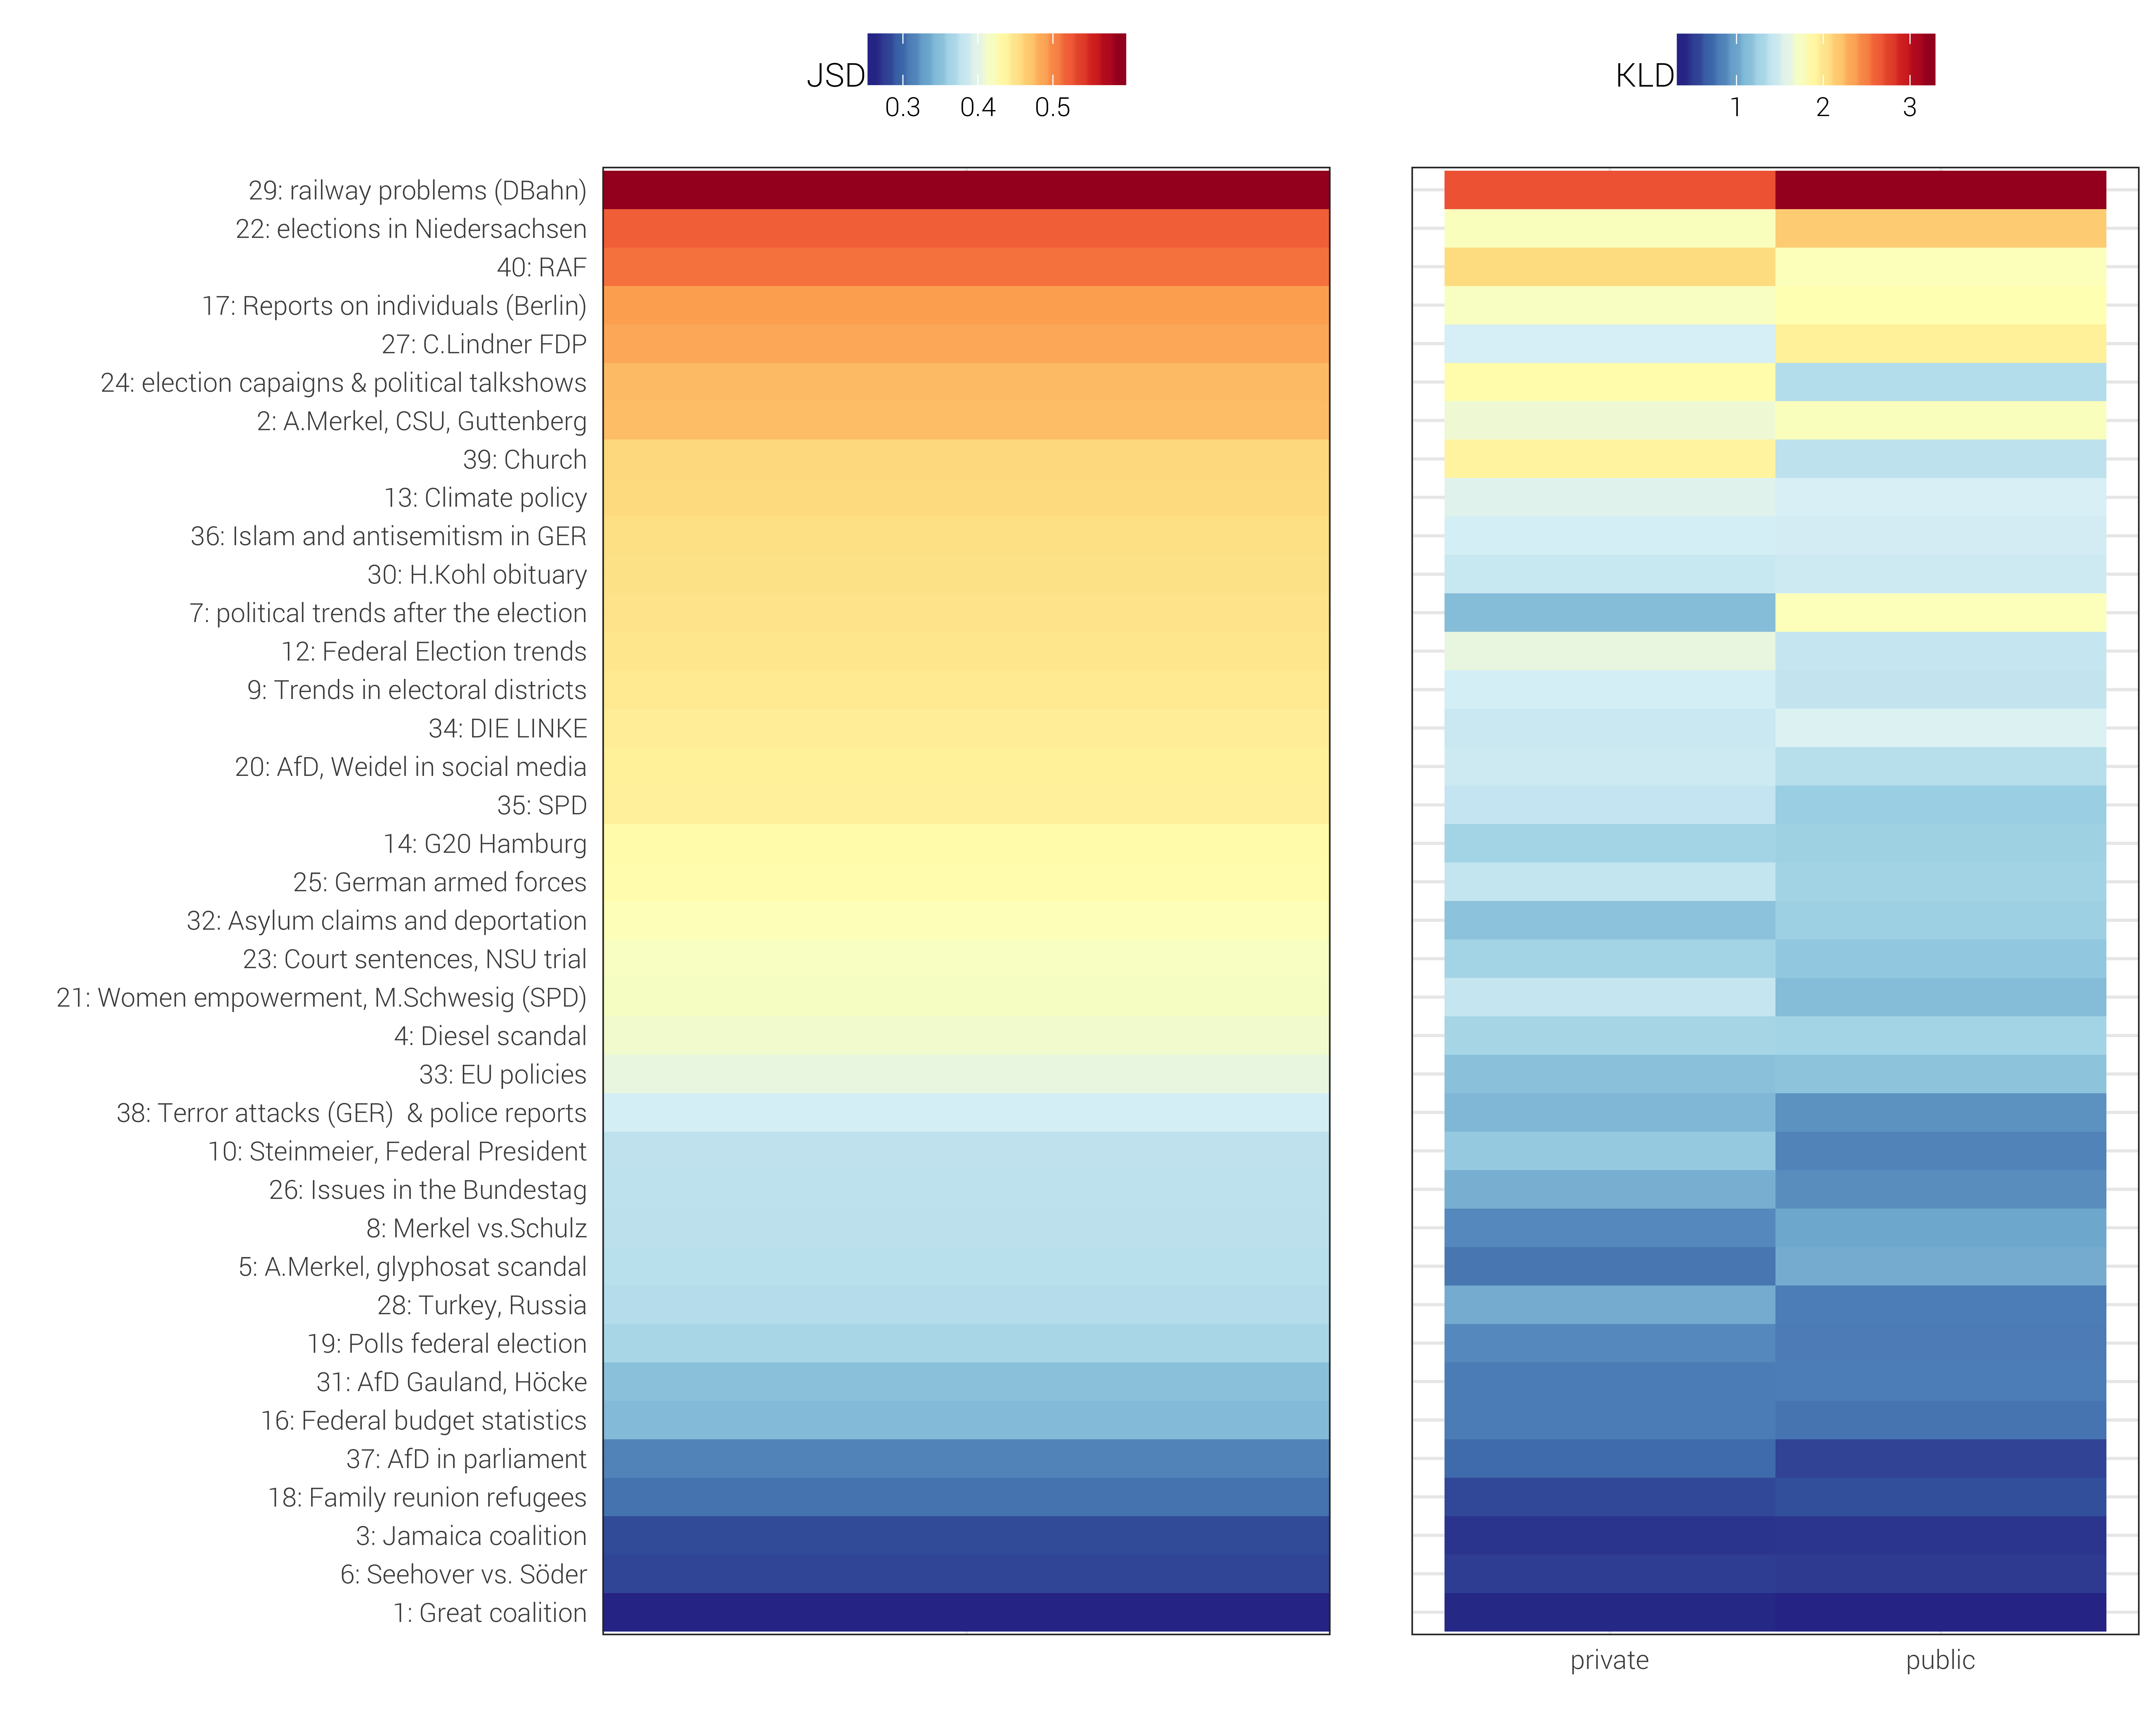
\includegraphics[width=\textwidth,keepaspectratio]{../figs/distance}
		\label{fig_distance}
	\end{center}
\end{figure}

\textcolor{red}{AUSWERTUNG}

% ----------------------
% Appendix
% ----------------------
\section*{Appendix}

\end{document}
